\documentclass{UoNMCHA}
\usepackage[authoryear]{natbib}
\usepackage{array,booktabs} % For nice tables
\usepackage{amsmath,amsfonts,amssymb} % For nice maths
\usepackage{color}
\usepackage{soul}       %for highlighting text
\usepackage{float}
\usepackage{enumerate}
\usepackage{listings}
\usepackage{caption}
\usepackage{subfig}
\usepackage{hyperref}
\usepackage{pdfpages}
\usepackage{setspace}
\usepackage{graphicx}
\usepackage[export]{adjustbox}
\usepackage[parfill]{parskip}   % For replacing paragraph indenting with a newline instead

% Number equations per section
\numberwithin{equation}{section}

\newcommand{\ra}[1]{\renewcommand{\arraystretch}{#1}}   %line spacing command tables use \ra{1.2}


\hypersetup{
%    bookmarks=true,         % show bookmarks bar?
%    unicode=false,          % non-Latin characters in AcrobatÕs bookmarks
%    pdftoolbar=true,        % show AcrobatÕs toolbar?
%    pdfmenubar=true,        % show AcrobatÕs menu?
%    pdffitwindow=false,     % window fit to page when opened
%    pdfstartview={FitH},    % fits the width of the page to the window
%    pdftitle={My title},    % title
%    pdfauthor={Author},     % author
%    pdfsubject={secject},   % subject of the document
%    pdfcreator={Creator},   % creator of the document
%    pdfproducer={Producer}, % producer of the document
%    pdfkeywords={keyword1} {key2} {key3}, % list of keywords
%    pdfnewwindow=true,      % links in new window
    colorlinks=true,       % false: boxed links; true: colored links
    linkcolor=black,          % color of internal links
    citecolor=black,        % color of links to bibliography
%    filecolor=magenta,      % color of file links
    urlcolor=black           % color of external links
}

\definecolor{MATLABKeyword}{rgb}{0,0,1}
\definecolor{MATLABComment}{rgb}{0.1328125,0.54296875,0.1328125}
\definecolor{MATLABString}{rgb}{0.625,0.125,0.9375}

\lstset{language=Matlab,
    basicstyle=\small\ttfamily,
    keywordstyle=\color{MATLABKeyword},
    %identifierstyle=,
    commentstyle=\color{MATLABComment},
    stringstyle=\color{MATLABString},
    numberstyle=\tiny,
    %numbers=left,
    basewidth=0.5em}

\firstpage{1}    % Set page number for first page
\UoNMCHAreportNo{MECH4841 Part B} %Report number
\UoNMCHAyear{2019}   % Year
\shorttitle{FYP Report - Acoustic Beamforming Array} %For odd pages
%%%%%%%%%%%%%%%%%%%%%%%%%%%%%%%%%%%%%%%%%%%%%%%%%%%%
\begin{document}
\singlespacing
\title{Proof of Concept Design of an Acoustic Beamforming Microphone Array for the Early Detection of Defects \\ \ \\
{\small Final Year Project Report - MECH4841 Part B  \\June 2020}}
\author[UoNMCHA]{Samuel Willis}
\address[UoNMCHA]{
Student of Mechanical Engineering,\\
The University of Newcastle, Callaghan, NSW 2308, AUSTRALIA \\
Student Number: 3256767 \\
E-mail: \href{mailto:s.willis@uon.edu.au}{\textsf{s.willis@uon.edu.au}}}
%%%%%%%%%%%%%%%%%%%%%%%%%%%%%%%%%%%%%%%%%%%%%%%%%%%%
\maketitle
\onecolumn
\newpage
\onehalfspacing
%%%%%%%%%%%%%%%%%%%%%%%%%%%%%%%%
\section*{Dot Point Summary}
    dot points that clearly articulates what you have achieved through your project. This is the 'no frills' run‐down of your project. This must be factual and defend able as it may well form the basis of questioning during your seminars.
    I developed,  created
\newpage
%%%%%%%%%%%%%%%%%%%%%%%%%%%%%%%%
\vspace{-5mm}
\section*{Abstract}
\vspace{-3mm}
    % https://student.unsw.edu.au/sample-abstracts-writing
    % Background Statement
    % Narrowing Statement
    % Elaboration of Narrowing Statement
    % Aims
    % Extended Aim
    % Results
    % Justification of Results/Future
    
    Locating defects and fault on plant can be difficult when a problem cannot be confidently diagnosed or located,
    now with the high availability of MEMS Microphones due to the ever-increasing demand of smartphones acoustic arrays consisting of large quantities of MEMS microphones have been made much more achievable without huge capital outlays. An array consisting of a large number of MEMS Microphones will allow for the beamforming of incoming signals and the locating of unknown sound sources. 
    
    The core aims of this project were to design and build an acoustic array consisting of up to 48 microphones that would be able to locate individual unknown sound sources from within a noisy environment for the purpose of locating defects in machinery by employing two different algorithms, the delay-and-sum and MUltiple SIgnal Classification (MUSIC). Once satisfied to be working the aim was to evaluate the performance of the acoustic array in detecting defects on in-service machinery in an industrial environment.
    
    The final array consisted of 24 microphones and proved to differentiate and locate multiple sound sources in a noisy environment using the MUSIC algorithm with ease, this algorithm allowed for the ability to target either a specific frequency or set of frequencies to spatially search for, easily differentiating sound sources. In the limited on-site testing at a local power station it was unable to determine the location of any noises present on an in-service turbine due to the harsh sound environment, though with further on-site testing and software refinement this array should be able to locate machine defects as it has shown in the lab environment.

%%%%%%%%%%%%%%%%%%%%%%%%%%%%%%%%
%%%%%%%%%%%%%%%%%%%%%%%%%%%%%%%%
\singlespacing
\newpage
\tableofcontents
\newpage
\listoftables
\listoffigures
\newpage
%%%%%%%%%%%%%%%%%%%%%%%%%%%%%%%%
%%%%%%%%%%%%%%%%%%%%%%%%%%%%%%%%
\section*{Nomenclature}
\subsection*{Latin Alphabet}
    \begin{table}[H]
        \begin{tabular}{clcl}
            $a$&Amplitude&$c$&Speed of sound\\
            $D$&Array diameter (Aperture)&$f$&Frequency\\
            $f_k$&Frequency Bin Frequency&$f_s$&Sample rate\\
            $k$&Frequency Bin&$K$&Number of Snapshots\\
            $M$&Number of Signals&$N$&Number of microphones\\
            $\mathbf{n}$&Noise Signal&$N_s$&Number of Samples\\
            $P_{\theta,\phi}$&Power at a point&$\mathbf{Q}_n$&Noise Subspace\\
            $\mathbf{Q}_s$&Signal Subspace&$r$&Signal source distance from origin of array\\
            $r_0$&Minimum array radius&$r_{max}$&Maximum array radius\\
            $\mathbf{R}$&Covariance Matrix&$\mathbf{R}_s$&Signal Covariance Matrix\\
            $s(t)$&Received signal&$\mathbf{S}$&Steering Vector\\
            $t$&Time&$T$&Temperature\\
            $v$&Underbrink Spiral angle&$x$&x-coordinate location of microphone\\
            $\mathbf{x}$&MUSIC Signal&$y$&y-coordinate location of microphone
        \end{tabular}
    \end{table}

    \subsection*{Greek Alphabet}
    \begin{table}[H]
        \begin{tabular}{cl}
            $\hat{\alpha}$&Narrow-band Signal\\
            $\lambda$&Wavelength\\
            $\tau$&Delay\\
            $\tau_s$&Delay in samples\\
            $\tau_\varphi$&Phase delay\\
            $\theta$&Azimuth angle\\
            $\phi$&Elevation angle\\
            $\varphi$&Phase\\
            $\varphi_A$&Steered azimuth angle\\
            $\varphi_E$&Steered elevation angle
        \end{tabular}
    \end{table}
%%%%%%%%%%%%%%%%%%%%%%%%%%%%%%%%
\newpage
\onehalfspacing
%%%%%%%%%%%%%%%%%%%%%%%%%%%%%%%%
\section{Introduction} \label{sec:Introduction}
    
    Beamforming is a technique where an array of sensors can be steered towards a particular direction either for transmission of signals or for the locating of signal sources \citep{Sha18}.
    
    The cocktail party effect, a phenomenon that relies on the human ability of being able to focus on one particular sound or voice when there are multiple other sources of noise, competing sources and distractions. This was first investigated in 1953 by Colin Cherry, what he referred to as the cocktail party problem, asking the question, can we replicate the ability of the cocktail party effect with man-made systems? This is the problem beamforming microphone arrays aims to solve \citep{Ben08}.
    
    For the purpose of this project beamforming is applied with an array of microphones being used to locate a sound source. Beamforming acoustic arrays are not a new concept, they have been used extensively in aerocoustics for the purpose of analysing aerofoils of aeroplanes and wind turbines for characterising and measuring generated noise as well as applications in finding the source of gas leaks, source of reverberation and general noise in studio environments, and finding squeaks and rattles in the automotive industry. One notable array is from a collaboration between Hyundai Motor Group and SM Instruments who together developed a small real-time acoustic array for the purpose of finding squeaks and rattles in Hyundai car's this array is available for purchase but costs upwards of \$65'000, though it's not suited for the purpose of early detection of defects on machinery especially as it can only beamform between the frequencies of 2kHz and 8kHz \citep{Smi}. The purpose of this project is to design an acoustic array to locate the sources of potential early defects in machinery for condition monitoring and analysis of plant.
    
%%%%%%%%%%%%%%%%%%%%%%%%%%%%%%%%
\newpage
\section{Literature Review} \label{sec:Literature Review}
%%%%%%%%%%%%%%%%%%%%%%%%%%%%%%%%
\subsection{Acoustic Beamforming} \label{sec:Beamforming}
    Through the digital processing of multiple signals received at microphones at known locations an estimated direction of arrival and location of a signal of interest can be found, this is the basic concept of acoustic beamforming. This process can be performed in either the time-domain or the frequency-domain by using different algorithms and processing techniques. One of the core assumptions for all algorithms is whether the audio waves are treated as far-field or near-field. The far-field assumption treats the sound waves as a planar wave-front while the near-field assumption treats sound waves as a spherical wave front. Sound waves can be assumed to be far-field when they have propagated such that Equation \ref{eq:propogate} is true \citep{McC01}, before this they are treated as near-field, this is due to point sources producing a spherical wave-front and as it propagates becoming planar \citep{Yan05}, a general rule of thumb can also be applied here, where far-field starts approximately 2 wavelengths from the sound source \citep{Mac19}. 
    
    \begin{equation}
        r > \frac{2D^2}{\lambda}
        \label{eq:propogate}
    \end{equation}
    \begin{table}[H]
    \centering
        \begin{tabular}{lrl}
            where, & $r$ &= Signal source distance from array origin \\
             & $D$ &= Array Diameter \\
             & $\lambda$ &= Wavelength (see Equation \ref{eq:wavelength})
        \end{tabular}
    \end{table}
    
    For the purpose of acoustic beamforming an array of microphones are used where the exact coordinate of each and every microphones is known and usually constant, the received signal at each sensor can then be synchronised, digitized and processed through a choice of algorithms and output the spatial location of a source of interest or audio from that point. This process involves using the known propagation speed of sound waves in air and the time difference of arrival for the signals at each one of the sensors.
    
    The geometry of the microphone array and the quantity of sensors becomes important for the accuracy and resolution of the estimated signal location. The choice of geometry arrangement whether it be in a grid, straight line or any other design can cause problems at particular frequencies due to spatial aliasing this will be further explained in Section \ref{sec:Signal Processing}, this requires careful consideration when designing the geometry of the microphone array, thus the frequencies of interest must be defined beforehand to determine the required microphone array design and size. These frequencies are particularly important for choosing the diameter of the microphone array (also known as the aperture) and the microphone spacing for grid and straight line arrays.
    
    Considerable amounts research and design have been achieved in the area of microphone array geometries, due to this several different array designs have been devised in attempt to increase the resolution and accuracy whilst avoiding spatial aliasing and minimising side-lobe levels as is discussed further in Section \ref{sec:2D Freq Response}. Some of the best performing and most popular array designs are shown in Figure \ref{fig:Mic Arrays}. These are regarded as some of the best performing due to them all having a high resolution with a high signal to noise ratio over a broad range of frequencies.
    
        \begin{figure} [H]
            \centering
            \begin{tabular}{cc}
                \subfloat[Archimedean Spiral]{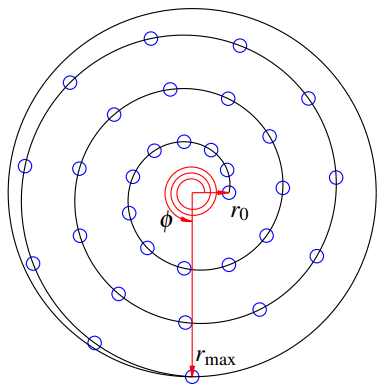
\includegraphics[keepaspectratio, width = 0.3\textwidth]{Figures/Archimedean.png}} &
                \subfloat[Dougherty Log-spiral]{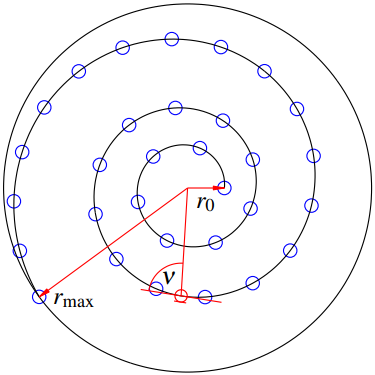
\includegraphics[keepaspectratio, width = 0.3\textwidth]{Figures/Dougherty.png}} \\
                \subfloat[Underbrink Array]{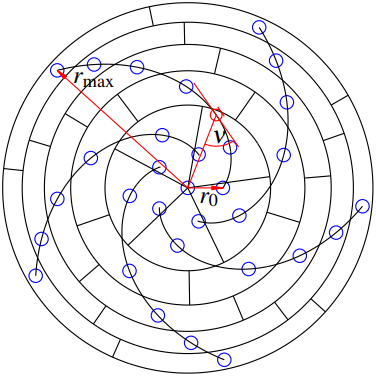
\includegraphics[keepaspectratio, width = 0.3\textwidth]{Figures/Underbrink.png}} &
                \subfloat[B\&K Array]{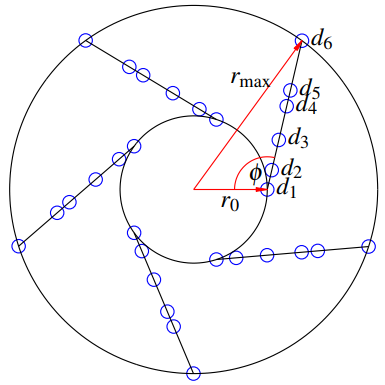
\includegraphics[keepaspectratio, width = 0.3\textwidth]{Figures/B&K.png}} 
            \end{tabular}
            \caption{Microphone Array Designs \citep{Pri13}.}
            \label{fig:Mic Arrays}
        \end{figure}
        
%%%%%%%%%%%%%%%%%%%%%%%%%%%%%%%%
\newpage
\subsection{Digital Signal Processing} \label{sec:Signal Processing}
    The processing of digital signals is the most important factor when it comes to beamforming, as an array of only two microphones have the potential to perform beamforming to a certain degree of accuracy, whilst improving the signal condition, signal processing, and choice of algorithm, the resulting accuracy can be improved.
    
    An analog signal is defined as a continuous signal that varies over time where the varying value in electronics is often voltage, for example the output of the microphones used throughout this project is a analog signal with a varying voltage between $\pm$ 50mV. Sampling of an analog signal is one of the core processes of digital signal processing, this is the process of discretization allowing the signal to be defined by a finite set of values. When sampling the signal it must be ensured that it is being sampled at a high enough rate to avoid aliasing, this is distortion that occurs when the reconstructed signal differs from the original due to not sampling at a high enough rate. This occurs when a signal is sampled at less than half of its the frequency, this required sampling rate is known as the Nyquist Rate. When sampled below the Nyquist Rate the audio waves are not able to be recreated accurately \citep{Ben08}. This concept is best explained with a visualisation, Figure \ref{fig:NyquistFrequency} shows one sine wave sampled at three different rates, from this we can see how if the sampling rate is equal to the frequency of the signal it esults in a constant amplitude whilst sampling at other frequencies below the Nyquist Rate will results in completely different signal with varying frequencies and amplitudes. 

    \begin{figure}[H]
        \centering
        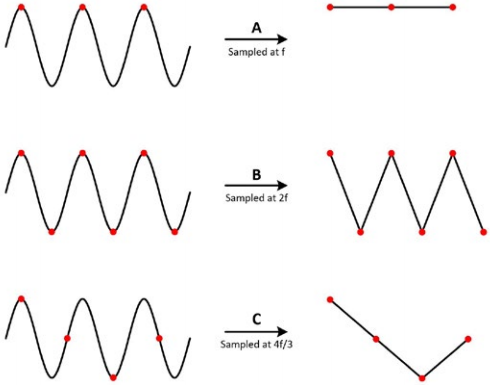
\includegraphics[keepaspectratio, width = 0.6\textwidth]{Figures/NyquistFrequency.png}
        \caption{Nyquist Rate Visualised \citep{NINyq}}
        \label{fig:NyquistFrequency}
    \end{figure}
    
    The concepts of a Nyquist rate and aliasing is directly related to Spatial Aliasing, this must be taken into account when designing microphone arrays. Spatial Aliasing occurs when the the location of the signal source cannot be determined due to the spacing of sensors in the microphone array relative to the wavelength of the signal of interest. This is similar to sampling and normal aliasing but rather than the points being sampled on the sine wave as being the problem its the spatial location of the microphones hence "spatial" aliasing. For example a $1000$Hz signal will have a wavelength of $34.3$cm shown by Equation \ref{eq:wavelength}, therefore if you have sensors spaced this distance apart it's not possible to tell exactly what direction the $1000$Hz signal is originating from, this can be explained as if you were to picture a signal at its peak at the first microphone it will also be at the peak for the second microphone, and therefore appear exactly the same, this is because they are exactly one wavelength apart, very similar to what is shown in Figure \ref{fig:NyquistFrequency}. For sensor arrays in a uniform line or grid the sensors must have a spacing of less than half the wavelength of the maximum frequency of interest to avoid spatial aliasing. An appropriately sized aperture is another important property of array geometry, the aperture is the diameter of the array and a larger aperture is required to beamform low frequency signals \citep{Ami08}.
	
	\begin{equation}
		\lambda = \frac{c}{f}
		\label{eq:wavelength}
	\end{equation}
	\begin{table}[H]
    \centering
        \begin{tabular}{lrl}
            where, & $c$ &= Speed of sound (see Equation \ref{eq:speed of sound}) \\
             & $f$ &= Frequency 
        \end{tabular}
    \end{table}
    
%%%%%%%%%%%%%%%%%%%%%%%%%%%%%%%
\subsubsection{Fourier Transform} \label{sec:Fourier Transform}

    The Fourier transform is a vital part of digital signal processing, especially for analysis of vibration signals and condition monitoring, as well as a requirement for beamforming in the frequency-domain. A Fourier Transform is used to change a signal from the time-domain to the frequency-domain. A signal in the time domain consists of a series of amplitudes with corresponding time-stamps, Fourier transforming will result in the signal being broken up into the individual frequencies that make up that signal, where each frequency is essentially a sinusoidal wave that have an individual amplitude and phase \citep{Sch17}. Figure \ref{fig:Fourier Transform} shows how a Fourier transform will break down a square wave signal, the red pane shows the original signal in the time-domain, the blue pane on the right shows the signal Fourier transformed spectrum, and in the middle we can see the actual individual waveforms the signal can be broken down into, this visualization allows us to see the frequency composition and the differing phases and amplitudes for each frequency.
    
    \begin{figure}[H]
        \centering
        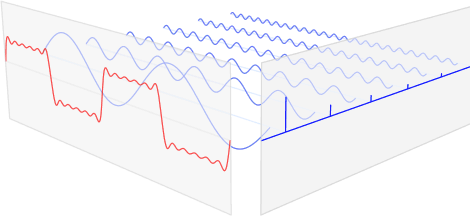
\includegraphics[keepaspectratio, width = 0.8\textwidth]{Figures/FFT.png}
        \caption{Fourier Transform Visualization.}
        \label{fig:Fourier Transform}
    \end{figure}
    
    The discrete Fourier transform is defined by Equation \ref{eq:DFT}, the core operation of the Fourier transform is the dot product. Performing a dot product of two equal length signals would be the equivalent multiplying them element by element and summing the result. The dot product result can be thought of as similarity, as the dot product of a sinusoidal wave and cosine wave of the same frequency will be 0, whilst two sinusoidal waves of the same frequency will be a maximum and two sinusoidal waves 180 degrees out of phase will be a negative maximum \citep{Sch17}. 
    
    \begin{equation}
        DFT[k]=\sum_{n-0}^{N_s-1}s[n] \cdot (cos(\varphi) - sin(\varphi)i)
        \label{eq:DFT}
    \end{equation}
        \begin{equation*}
        Where \; \varphi = k \frac{n}{N_s}2 \pi
    \end{equation*}
    
    When performing a Fourier transform on a finite length signal the resolution of the Fourier transform depends on the length and sampling rate of the digitized signal, due to this we have frequency bins which is the resolution of the Fourier transform and therefore frequency spectrum, if the spectrum begins at 0 and the frequency bin size is 4Hz this would mean all of the frequencies from 0 to 4Hz would essentially be summed into the single bin at 4Hz, and frequencies from 4 to 8Hz would be in the 8Hz bin and so on. From Eqn. \ref{eq:DFT} we define $N$ as the number of samples in a signal and $k$ as a frequency bin, as the output of a discrete Fourier Transform is a series of frequency bins. Each one of the $k$ output frequency bins corresponds to a particular frequency that can be calculated with Equation \ref{eq:freq bin}, the result when $k=1$ is the size of the frequency bins.
    
    \begin{equation}
        f_k = k \times \frac{sample\;rate}{N_s}
        \label{eq:freq bin}
    \end{equation}
    
    As can be determined by Equation \ref{eq:freq bin} the resolution of the discrete Fourier Transform relies on the amount of time of the signal is processed, 1 second signal will have 1Hz frequency bins whilst 0.25 second signal will have 4Hz frequency bins and hence the frequencies within the 4Hz range will be effectively summed together into each frequency bin.
    
%%%%%%%%%%%%%%%%%%%%%%%%%%%%%%%
\subsubsection{Delay-and-Sum Beamformer} \label{sec:DAS Algorithm}
    The Delay-and-Sum algorithm is the classical method of beamforming in the time-domain and one of the most robust and well used. As the location of each sensor in the array is known and we know that sound waves propagate at the speed of sound, we can determine that a distant sound source of will arrive at each sensor at a slightly different time this is the time difference of arrival that is calculated with the array geometry and is the core of all methods beamforming.
    
    The name of this algorithm comes from the processes undertaken, consisting of two main steps; delaying and summing. First the signal from each sensor is individually shifted by a time delay that corresponds to a particular spatial location relative to the sensor, the signals are then summed to receive the resulting waveform from that location \citep{GreWeb} this process is digitally steering the microphone array. Once the resulting signal is divided through by the number of sensors we have attenuated and amplified the signal at the angle of interest and dulled signals from all other locations as they will not interfere constructively. This concept is visually demonstrated in Figure \ref{fig:das-diagram}, showing how the angle of interest is attenuated in comparison to all other angles being dulled.
    
    \begin{figure}[H]
        \centering
        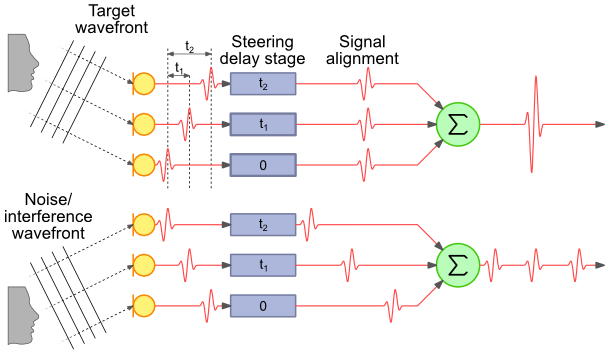
\includegraphics[keepaspectratio, width = 0.8\textwidth]{Figures/DAS-Diagram.png}
        \caption{Delay-and-Sum Beamforming Diagram \citep{GreWeb}.}
        \label{fig:das-diagram}
    \end{figure}
%%%%%%%%%%%%%%%%%%%%%%%%%%%%%%%%
\subsubsection{Frequency-Domain Beamformer} \label{sec:Freq-Domain Beamformer}
    Delay-and-Sum beamforming is performed in the time-domain as the signal is a function of amplitude and time, there are other algorithms that are used in the time-domain based off of delay-and-sum theory, though there are several other algorithms that process in the frequency-domain. Beamforming in the frequency-domain involves analysing the signals by their amplitudes of individual frequency bins without respect to time but to the signal as a whole and therefore must be over a set period of time. 
    
    A conventional frequency-domain beamformer requires the incoming signal to be in the Fourier-domain which is achieved by performing a Fourier transform as described in Section \ref{sec:Signal Processing}. Compared to the time-domain delay-and-sum beamformer where the signal is delayed by shifting/delaying the times of the incoming signals the frequency-domain differs, the signal is delayed by adding a phase delay to the individual frequency bins that are a result of the Fourier transform, this theoretically achieves the same result as the delay-and-sum beamforming but has the advantage of being far less computationally intensive and potentially have far greater accuracy in results. \citep{Kri13}.

%%%%%%%%%%%%%%%%%%%%%%%%%%%%%%%%
\subsubsection{MUSIC Algorithm} \label{sec:Intro MUSIC}
    The MUltiple SIgnal Classification algorithm (MUSIC) is a subspace frequency-domain method of beamforming relying upon an eigen-decomposition of the spatial co-variance matrix of the received signal data. The spatial co-variance matrix is decomposed into it's eigenvalues and vectors that are then sorted by eigenvalue and separated into noise and signal subspaces.
    With the use of array steering vectors based on phase rather than time, the direction of arrival can be estimated as the steering vector is theoretically orthogonal to the noise subspace obtained from eigenvalue decomposition and therefore when multiplied together results in 0 \citep{Pau} \citep{MatL}, when taking the reciprocal of this it will tend towards infinity when at the angle of the sound source similar to what is seen in Figure \ref{fig:das music comparison}. This results in a high resolution algorithm for estimating the direction of arrival of either narrowband or wideband signals and far less computationally heavy compared to the traditional Delay and Sum beamforming algorithms. Below in Figure \ref{fig:das music comparison} a comparison of the two algorithms is shown for the purpose of demonstrating the additional resolution and accuracy gained. 

    % \hl{What is subspace? covariance?}

    \begin{figure}[H]
        \centering
        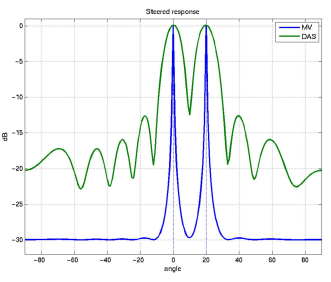
\includegraphics[keepaspectratio, width = 0.6\textwidth]{Figures/DASMUSICcomparison.png}
        \caption{MUSIC and Delay and Sum Comparison \citep{Nas12}.}
        \label{fig:das music comparison}
    \end{figure}
    
%%%%%%%%%%%%%%%%%%%%%%%%%%%%%%%%
    \subsection{Condition Monitoring} \label{sec:Condition Monitoring}
    "Condition monitoring is the continuous monitoring of rotating machines during process conditions. This ensure the optimal use of machines. Condition Monitoring supports predictive maintenance, which is more efficient than preventive maintenance. Condition Monitoring provides insight in performance, wear and mechanical risks of machines. This helps to prevent unnecessary and unplanned downtime."\citep{Ist}.
    
    Preventive maintenance of machinery is the regular replacement of components based on a rigid schedule and the typical operating life expectations resulting in parts being replaced or lubricated more often than necessary to meet these requirements resulting in inefficient use of valuable time. With the introduction of electronic instrumentation allowing vibration analysis and potentially acoustic analysis these preventive maintenance programs can be easily converted to predictive maintenance programs. Predictive maintenance uses data from measurements and other analysis performed on a regular basis, the concept is to predict when it is necessary to take the machine out of service for maintenance and/or repair rather than waiting for the machine to breakdown and require fixing, this leads to an effective and efficient maintenance program \citep{Laws87}.
    
    Condition Monitoring is part of the maintenance program though relates more to a particular machine. Condition Monitoring aims to define the current condition of a machine by comparing it to previously known conditions. Analysing the trends of this allows for the prediction of machine condition over time. Through the use of an acoustic array that could potentially be permanently setup the condition of the machine can be easily monitored and any changes or particular noises will be able to be analysed individually or montioring could be done on a routine basis to analyse trends in the machinery sound-scape.
%%%%%%%%%%%%%%%%%%%%%%%%%%%%%%%%
\newpage
\section{Aims and Objectives} \label{sec:Aims and Objectives}
%%%%%%%%%%%%%%%%%%%%%%%%%%%%%%%%
\subsection{Problem} \label{sec:Problem}
    Currently the condition monitoring of rotating machinery is primarily performed using vibration, proximity and temperature sensors. This is generally performed on a schedule with routine data analysis for insight into any trends or patterns indicating machinery may need additional maintenance or repair. If this machine in the mean-time starts to make odd noises from an unknown location it can be a lengthy and expensive process to determine where it is coming from and why. With an acoustic array set up in-front of machinery it is possible to monitor a large area for any changes in sound or appearance of problem noises and therefore will be able to identify where the problem has arisen from, even further it will be possible to analyse the noise further and potentially diagnose the problem. This could potentially save a great amount of time and money especially if other techniques require machinery to be taken out of service for analysis.
%%%%%%%%%%%%%%%%%%%%%%%%%%%%%%%%
\subsection{Use of Microphone Arrays for Condition Monitoring} \label{sec:use for CM}
    Currently there are few acoustic arrays that have been built for the purpose of condition monitoring, they have been shown to be a powerful tool with serious potential in an article on the analysis of electric motors with an acoustic camera \citep{Orm13}. There is one acoustic technology company "Squarehead Technology" that offer condition monitoring acoustic arrays as one of their services in the USA and Norway but besides this there is a large gap in the market of acoustic arrays purpose built for condition monitoring especially for outright purchase. With the ability to choose how the algorithms are processing the incoming data it will give the ability to pinpoint the locations of individual machine defects through the known fault frequencies and harmonics.
%%%%%%%%%%%%%%%%%%%%%%%%%%%%%%%%
\subsection{Project Aim} \label{sec:Project  Aim}
    By the completion of my final year project I aim to have a completely functioning acoustic array. This array should be able to determine when a noise of interest is present, locate it spatially and return a clean signal for further analysis. The current milestones are as follows:
    
    \begin{itemize}
        \item Learn about audio signal processing and developed a greater understanding.
        \item Develop an understanding of condition monitoring, vibration analysis and its application.
        \item Learn LabVIEW and Develop a greater understanding of data acquisition and software development.
        \item Develop a simulation environment for quick and easy testing of array geometries and beamforming algorithms.
        \item Implement a working algorithms in both the time and frequency domain and show it working in simulation.
        \item Build an acoustic array using NI Hardware and MEMS Microphone.
        \item Show a working acoustic array able to locate and detect sounds.
        \item Show the acoustic array picking particular sounds out of noisy environments.
        \item Extract the signal from point of interest for further analysis.
        \item Test the acoustic array on site on operating machinery.
    \end{itemize}
    
    With a working acoustic array it will allow for the optimisation of the maintenance and monitoring for a large range of machinery improving the financial costs, time and safety as well as analysis for early detection of defects and locating of unknown sources of noises.
%%%%%%%%%%%%%%%%%%%%%%%%%%%%%%%%
\newpage
\section{Software Research and Development} \label{sec:Software}

    LabVIEW by National Instruments was the chosen environment for software development and data acquisition. This choice was made due to the integration with National Instruments' Hardware that was readily available for the purpose of this project. 
    
    LabVIEW is short for Laboratory Virtual Instrument Engineering Workbench, a programming environment in which you create programs graphically connecting function blocks with wires for data flow. LabVIEW features a graphical user-interface making it simple for simulations, presentation of ideas and general programming \citep{Tra06}. With the inbuilt digital signal processing and data acquisition libraries this makes LabVIEW incredibly useful for the purpose of developing an acoustic array.
%%%%%%%%%%%%%%%%%%%%%%%%%%%%%%%%
\subsection{Delay-and-Sum Algorithm} \label{sec:Software DAS}
    To begin a full investigation into acoustic beamforming arrays a complete understanding of the delay-and-sum beamformer is required. For explanation and ease of understanding it is best to think of a uniform linear array of $N$ microphones (sensors). Figure \ref{fig:ULA} demonstrates a uniform linear array, where $s(t)$ is an unknown sound source impinging on the array from the far-field as a planar wavefront, $\theta$ is the incoming incident angle of the unknown source, $d$ is the spacing between sensors, $v_n(t)$ is additive noise and interference from the environment, $x_n(t)$ is the signal at each sensor, and $y_n(t)$ the output of each of these sensors.
    
    \begin{figure} [H]
        \centering
        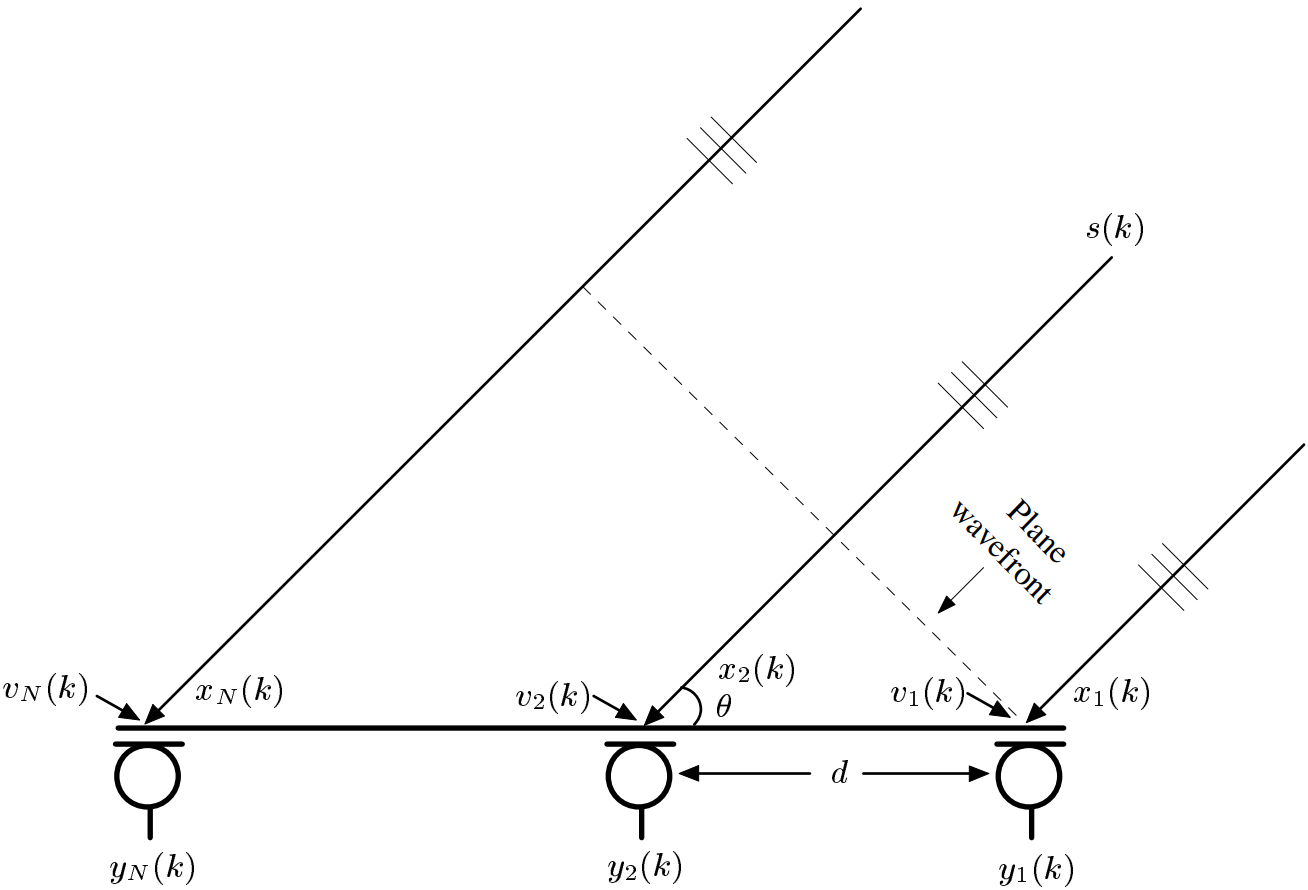
\includegraphics[keepaspectratio, width = 0.8\textwidth]{Figures/ULA.png}
        \caption{Uniform Linear Array of Microphone Array \citep{Ben08}.}
        \label{fig:ULA}
    \end{figure}
    
    As can be seen in the diagram, the path to each microphone has slightly differing lengths, this is what causes the differing time delays and allows for beamforming as it is the fundamental reason beamforming is possible. If we let $\mathbf{s}(t)$ be the received signal at the origin then an array of signals received at each sensor at time instant $t$ is written as seen in Eqn \ref{eq:signal array} and $s_n(t)$ will be the signal received at sensor $n$:
    
    \begin{equation}
        \mathbf{s{(t)}} = [s(t-\tau_1), s(t-\tau_2), ..., s(t-\tau_N)]^T
        \label{eq:signal array}
    \end{equation}
    \begin{equation}
        s_n(t) = s(t-\tau_n)
        \label{eq:sensor signal}
    \end{equation}
    
    In Equation \ref{eq:signal array}, $\tau$, is the time delay, also known as the time difference of arrival, as it is the difference in time for the signal to reach microphone $n$ relative to a reference microphone or the centre of the array. For arrays of any geometry this delay can be quite easily calculated using trigonometry, the speed of sound, and location of the sensors. It should always be taken into account that the speed of sound in air will change with the temperature, $T$, this relationship is shown in Equation \ref{eq:speed of sound}. 
    
    \begin{equation}
        c = 331.3 \times \sqrt{1+\frac{T}{273.15}}
        \label{eq:speed of sound}
    \end{equation}
    
    For the uniform linear array we can find the delay for each microphone using the respective $x$ locations relative to the origin at the centre of the microphone array and the Equation \ref{eq:TDOA}.
    
    \begin{equation}
        \tau = \frac{x\cdot cos(\theta)}{c}
        \label{eq:TDOA}
    \end{equation}
    
    This can be modified for 2D planar arrays so that it takes into account the $x$ and $y$ location  relative to the origin at the centre of the microphone array, by using Equation \ref{eq:TDOAx+y}, this will allow the use of any array of microphones, including the arrays pictured in Figure \ref{fig:Mic Arrays}.
    
    \begin{equation}
        \tau = \frac{x \cdot cos(\theta) + y \cdot sin(-\phi)}{c}
        \label{eq:TDOAx+y}
    \end{equation}
    
    Both Equation \ref{eq:TDOA} and \ref{eq:TDOAx+y} make the assumption of, the azimuth ($\theta$) being the angle sweeping across horizontally in-front of the array ranging from $0^{\circ} \to 180^{\circ}$ where $90^{\circ}$ is at the origin and the elevation ($\phi$) sweeping from the bottom at $-90^{\circ}$ to the top at $90^{\circ}$ vertically. This co-ordinate system is used to digitally steer the beam over a virtual area in-front of the array to determine where a signal is coming from by iterating through all combinations of azimuth and elevation. The point in-front of the array where the signal has the highest equivalent power is the estimation of the signal source's location.
    
    Using this delay-and-sum algorithm will also allow for the extracting of signals from a particular spatial location by applying the algorithm to a single spatial point rather. For the point of interest the channels are delayed accordingly, summed and then divided by the number of microphones to return a single waveform for the location of interest.
%%%%%%%%%%%%%%%%%%%%%%%%%%%%%%%%
\subsubsection{LabVIEW Implementation} \label{sec:DAS Implementation}
    For the real implementation of the delay-and-sum algorithm the delay equation needs a minor modification due to the digital sampling of signals. For instance when a signal is sampled at $30$kHz known as the sample rate ($f_s$), the time between each sample is approximately $0.033$ms, now we have to work in discrete time steps of this sample length rather than continuous time, therefore the delay formula is re-written as shown in Equation \ref{eq:TDOAfs} to take this into account.
    
    \begin{equation}
        \tau_s = \frac{x \cdot cos(\theta) + y \cdot sin(-\phi)}{c}\cdot f_s
        \label{eq:TDOAfs}
    \end{equation}
    
    A problem arises using Equation \ref{eq:TDOAfs} when the calculated delay for a particular channel is not an integer, due to the digital sampling the smallest delay is the sample length as it is not possible to delay by sub-sample time steps. When using a lower sampling rate this problem can cause large inaccuracies, the easiest way to prevent this is to use the highest possible sample rate to minimise the error, otherwise, the incoming signal can be up-sampled by a preset factor using a Linear Up-sampler or Finite Impulse Response Filter, this up-sampling factor is taken into account with the delay by multiplying the original sampling rate by this same factor. 
    
    The process in LabVIEW for applying the delay to each signal was to find the largest and the smallest delay required for that particular point, then for each channel the absolute value of the smallest delay for that point plus the individual channel delay worth of zeroes are added to the beginning of the signal as padding. Following this, the absolute value of the largest delay of samples are removed from this signal to ensure there are no zeroes left in the signal to keep signal integrity. The LabVIEW code for this process is shown in Figure \ref{fig:DelayLabVIEW}, as can be seen LabVIEW code is closer to a block-diagram than traditional text-based programming languages. The two rectangular structures in Figure \ref{fig:DelayLabVIEW} are For Loops, the outer loop iterates through a larger 2D array of delays and returns a 1D array of delays for a particular azimuth and elevation, the inner loop iterates through a 1D array of each channel applying the correct delay channel by channel.
    
    \begin{figure} [H]
        \centering
        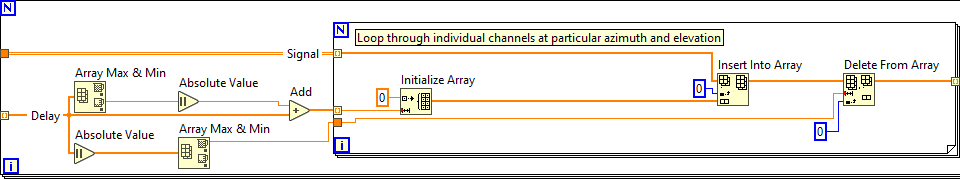
\includegraphics[keepaspectratio, width = \textwidth]{Figures/DelayBlockDiagram.png}
        \caption{LabVIEW Delay Block Diagram Data Flows Left to Right}
        \label{fig:DelayLabVIEW}
    \end{figure}
    
    To produce a heat-map of the location of sounds in-front of the acoustic array the array is digitally steered to each point on a virtual grid in-front of the array and the equivalent power of the signal at this point is evaluated then plotted. For the delay-and-sum beamformer this process involves going through each azimuth and elevation giving a grid 180 by 180 points representing the area in-front of the array and delaying and summing at each point. The analog signals once digitized are converted to an array of floating point values where each index is an individual sample of amplitude, then for each point on the array the signal is to be delayed by the calculated amount using Equation \ref{eq:TDOAfs}, then an equivalent power at each point is calculated as a single number, using Equation \ref{eq:power}, this produces a 2D array that is plotted as an intensity or heat-map.
   
    \begin{equation}
        P_{(\theta, \phi)} = \sum_{t=0}^\infty\Big(\frac{\sum_{n=1}^N x_n(T)}{N}\Big)^2
        \label{eq:power}
    \end{equation}
    \begin{equation*}
        where,\;x_n(T) = x_n(t-\tau_{s,n})
    \end{equation*}
    
    Equation \ref{eq:power} determines the power at a single point by summing all the channels at that point resulting in a single signal wave that has been either constructively and destructively interfered then divided by the number of channels normalising the resulting waveform, an example of this can be seen in Appendix \ref{app:Sim}. Now the single interfered waveform is squared element-by-element, this process makes all values positive but also attenuates the peaks of the signal relative to the troughs. Finally each amplitude value for every sample of the wave is summed together resulting in a single value for that point. This process makes sure positions with larger amounts of constructively interfered signals that are closer to the signal location are attenuated further and return a higher value allowing for a heat-map to be created with the estimated signal source location. So that the heatmap could be easily interpreted the output 2D array of power of the grid is re-scaled between 1 and -1 for easy interpretation therefore if the value for a location is 1 it is the most likely estimation of the location of the signal of interest.
    
%%%%%%%%%%%%%%%%%%%%%%%%%%%%%%%%
\subsection{MUSIC Algorithm} \label{sec:Software MUSIC}
    This section has been adapted from Direction of Arrival Estimation \citep{Adv13} and DOA Estimation based on MUSIC algorithm \citep{Tan14} for this project. When approximating the direction of arrival of signals using the multiple signal classification algorithm the anticipated data for the $M$ arriving signals are modeled as below in Eqn. \ref{eq:MUSIC signal}.
    
    \begin{equation}
        \mathbf{x}=\mathbf{S\hat{\alpha}} + \mathbf{n}
        \label{eq:MUSIC signal}
    \end{equation}

    $\mathbf{S}$ is a $N \times M$ array consisting of a series of steering vectors for the M impinging signals. $\hat{\alpha}$ is a vector of the narrowband signals impinging on the array that consists of each signals amplitude and phase. $\mathbf{n}$ is a vector consisting of the noise received at each of the microphones which is assumed to be a zero-mean Gaussian distribution with a co-variance of $\sigma^2I$.

    \begin{equation}
        \mathbf{S}=
        \begin{bmatrix}
            \mathbf{s}(\theta_1,\phi_1) & \mathbf{s}(\theta_2,\phi_2) & \cdots & \mathbf{s}(\theta_M,\phi_M)
        \end{bmatrix}
    \end{equation}
    \begin{equation}
        \hat{\alpha}=
        \begin{bmatrix}
        \alpha_1 & \alpha_2 & \cdots & \alpha_M
        \end{bmatrix}
        ^T
    \end{equation}
    Where:
    \begin{equation}
        s(\theta,\phi)=e^{-j2\pi \tau(\theta,\phi) f}
    \end{equation}
    \begin{equation}
        \alpha = ae^{\varphi}
    \end{equation}
    
    An assumption is made that the impinging signals are uncorrelated, and therefore the estimated correlation of matrix of $\mathbf{x}$ is as shown in Eqn. \ref{eq:covariance}, in this $E[\;]$ represents the expected value and $H$ is the notation used to indicate a hermitian or conjugate transpose of the array. A conjugate transpose involves transposing the array and also taking the conjugate of the complex conjugate of all values.
    
    \begin{equation}
    \begin{split}
        R & =  E[\mathbf{xx}^H] \\
        & = E[\mathbf{S\hat{\alpha}\hat{\alpha}}^H\mathbf{S}^H] + E[\mathbf{nn}^H] \\
        & = \mathbf{SAS}^H + \mathbf{\sigma^2I}\\
        & = \mathbf{R}_s + \mathbf{\sigma^2 I}
    \end{split}
    \label{eq:covariance}
    \end{equation}
    where
    \begin{equation}
        \mathbf{R_s} = SAS^H
    \end{equation}
    \begin{equation} 
    \mathbf{A} = 
    \begin{bmatrix}
        E[|\hat{\alpha}_1|^2] & 0 & \dotsm & 0\\ 
        0 & E[|\hat{\alpha}_2|^2] & \dotsm & 0\\ 
        \vdots & \vdots & \ddots & \vdots\\ 
        0 & 0 & \dotsm & E[|\hat{\alpha}_M|^2]
    \end{bmatrix}
    \end{equation}
    
    $\mathbf{R}_s$ is the signal co-variance matrix, an $N \times N$ array that has rank $M$. When performing eigen-decomposition of the signal co-variance matrix $\mathbf{R}$ it results in $N$ eigenvalues and eigenvectors, there are $N - M$ eigenvalues and corresponding vectors that span the noise subspace $\mathbf{Q}_n$, and $M$ spanning the signal subspace $\mathbf{Q}_s$.
    The eigenvalues and corresponding vectors are then sorted in descending order of eigenvalue. The $N-M$ eigenvalues that should be equal to $\sigma^2$ are the eigenvalues that span the noise subspace and those eigenvalues corresponding vectors create the matrix $\mathbf{Q}_n$. If we let $\mathbf{q}_m$ be one of the eigenvectors corresponding to the noise subspace we can show,
    
    \begin{equation}
    \begin{split}
        \mathbf{R}_s\mathbf{q}_m = \mathbf{SAS}^H\mathbf{q}_m & = 0\\
        \therefore \; \mathbf{q}_m^H\mathbf{SAS}^H\mathbf{q}_m & = 0
    \end{split}
    \end{equation}

    This implies that the noise eigenvectors are orthogonal to the $M$ steering vectors and is the basis of the MUSIC algorithm. Where orthogonal vectors are those whose dot product equals $0$, if plotted in 2D these would be perpendicular \citep{Wei}.
    
    Once the noise subspace matrix $\mathbf{Q}_n$ has been determined the MUSIC pseudo spectrum of power can be calculated as a function of $\theta$ and $\phi$ as shown in Eqn. \ref{eq:MUSIC Power}, as shown above due to the fact that the noise eigenvectors are orthogonal to the steering vectors when the the azimuth and elevation are that of the impinging signal and therefore Eqn. \ref{eq:MUSIC Power} will get exponentially larger as the correct location for the signal is found.
    
    \begin{equation}
        P_{MUSIC}(\theta,\phi) = \frac{1}{\mathbf{s}^H(\theta,\phi)\mathbf{Q}_n\mathbf{Q_n}^H\mathbf{s}(\theta,\phi)} = \frac{1}{||\mathbf{Q}_n^H\mathbf{s}(\theta,\phi)||^2}
        \label{eq:MUSIC Power}
    \end{equation}

%%%%%%%%%%%%%%%%%%%%%%%%%%%%%%%%
\subsubsection{LabVIEW Implementation} \label{sec:MUSIC LabVIEW}
    When implementing the MUSIC algorithm in LabVIEW I started with the narrowband MUSIC approach where it is assumed the signal only contains a single frequency $f$ the same as is outlined in Section \ref{sec:Software MUSIC}.
    
    Firstly the complex phase delays for each microphone in the array were generated for every combination of elevation and azimuth in front of the array. These were calculated using equations \ref{eq:AzEl TDOA} and \ref{eq:Complex Phase Delay}.
    
    \begin{equation}
        \tau_n(\theta, \phi) = \frac{x \cdot cos(\theta) + y \cdot sin(-\phi)}{c}
        \label{eq:AzEl TDOA}
    \end{equation}
    \begin{equation}
        \mathbf{s}_n(\theta,\phi) = exp(-j \cdot 2\pi \cdot \tau \cdot f)
        \label{eq:Complex Phase Delay}
    \end{equation}
    \begin{equation*}
        For \; n = 1,2,...,N
    \end{equation*}
    
    Next the correlation matrix is calculated for $\mathbf{x}$, the true value is not able to be calculated and must be estimated, the estimation is made using the received data from the microphone array, this is performed by averaging the result over several snapshots of data as can be seen in Eqn. \ref{eq:covariance average} the rule of thumb is that $K > 2N$ for the number of averages required \citep{Adv13}, by performing averaging it allows for a more accurate representation of the noise and signal subspace. 
    
    \begin{equation}
        \mathbf{R} = \frac{1}{K}\sum_{k=0}^K\mathbf{x}_k\mathbf{x}_k^H
        \label{eq:covariance average}
    \end{equation}

    
    To get the value for $\mathbf{x}_k$ the length of the incoming signals from each array in samples is determined, the signal for each channel is then divided into $K$ equal snapshots of equal length. A Fourier transform is performed for each snapshot for each channel and the value of the complex spectrum for the particular narrowband frequency $f$ is returned for each channel and snapshot. As the signal is being broken up into $K$ snapshots the returned value for the complex spectrum may not be only for the narrowband of $f$ and rather will be the value for the closest frequency bin to the frequency $f$ as was outline in Section \ref{sec:Fourier Transform}.
    
    Now with $K$ vectors of $\mathbf{x}$, the correlation matrix can be calculated for each snapshot and then averaged, this gives an estimation for the real correlation matrix.
    
    Once the correlation matrix has been estimated eigenvalue decomposition is performed. This returns $N$ eigenvalues, and eigenvectors, these are sorted in descending order and split into the signal and noise subspace. The $N-M$ eigenvectors corresponding to the $N-M$ smallest eigenvalues the matrix $\mathbf{Q}_n$, in the software implementation of MUSIC the $N-M$ eigenvalues should be the smallest and all roughly equal. Now applying Eqn. \ref{eq:MUSIC Power} the direction of arrival for the $M$ signals can be determined by the peaks in the equation. 
    
    Below Figure \ref{fig:MUSICBlockPt1} and \ref{fig:MUSICBlockPt2} show the LabVIEW block diagrams of one of my implementation of the MUSIC algorithm, in particular wideband MUSIC through a given range of frequencies. Figure \ref{fig:MUSICBlockPt1} shows the process of iterating through each channel and then for each snapshot the complex spectrum value is calculated as well as the microphone delay matrix.
    
    \begin{figure}[H]
        \centering
        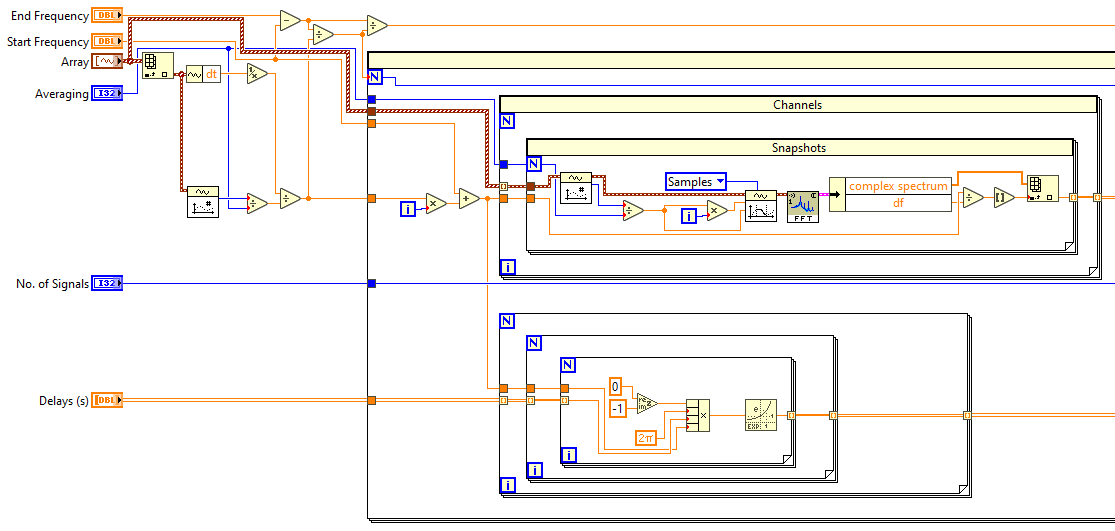
\includegraphics[keepaspectratio, width = 0.99\textwidth, frame]{Figures/MUSCBlockPt1.png}
        \caption{LabVIEW MUSIC Implementation Block Diagram Pt.1}
        \label{fig:MUSICBlockPt1}
    \end{figure}
    
    Figure \ref{fig:MUSICBlockPt2} shows the calculating of the correlation matrix for each snapshot, the averaging of this, the eigen-decomposition of the estimated correlation matrix over the $K$ snapshots and the calculation of the MUSIC power spectrum following the process that has been described above.

    \begin{figure}[H]
        \centering
        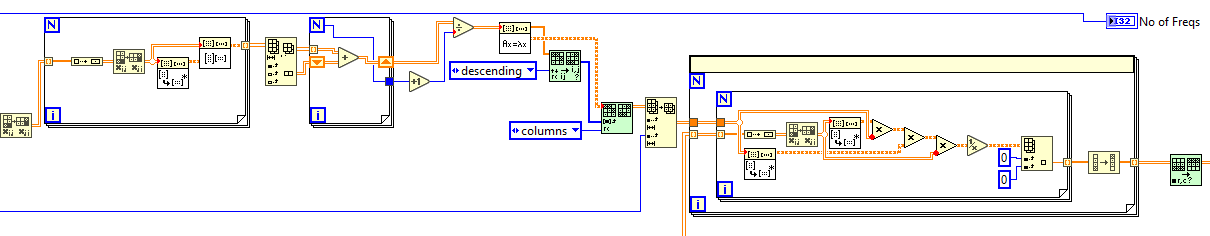
\includegraphics[keepaspectratio, width = 0.99\textwidth, frame]{Figures/MUSICBlockPt2.png}
        \caption{LabVIEW MUSIC Implementation Block Diagram Pt.2}
        \label{fig:MUSICBlockPt2}
    \end{figure}
    
    When applying the MUSIC algorithm to a wideband signal instead of a single frequency there will almost definitely be multiple frequencies all belonging to the same frequency bin, if the algorithm was to iterated through every single frequency and solve this would increase the computational effort required dramatically as it could be required to iterate through hundreds of unnecessary frequencies. To reduce the computational requirements the size of the frequency bins of the Fourier transform for each snapshot are calculated using the following Eqn. \ref{eq:FreqBin} where $N_s$ is the number of samples in the full signal.
    
    \begin{equation}
        f_{k} =\frac{f_s \cdot K}{N_s}
        \label{eq:FreqBin}
    \end{equation}
    
    Once the size of the frequency bins are established the wideband frequency range is then divided by the bin size to determine how many iterations/FFTs are required as then rather than iterating through each individual required frequency, iterations are done by frequency bin. For each frequency bin the full narrowband compute as described above is calculated and the resulting power for each frequency at each point is averaged to calculate the estimated direction of arrival of the $M$ wideband signals.
    
    Identical to the 2D array of power returned by the delay-and-sum the MUSIC algorithm returns a value for each spatial location using equation \ref{eq:MUSIC Power} which is normalised between -1 and 1, again with 1 being the most likely location of the signal of interest to allow direct comparison to the delay-and-sum algorithm and easy interpretation of results. The one downside of MUSIC compared to the delay-and-sum algorithm the MUSIC algorithm does not actually resolve a resultant signal at each location and therefore cannot be used to extract signal without the help of delay-and-sum. 
    
    Another very useful implementation of the MUSIC algorithm is using a select number of pre-determined frequencies to perform the average over for rather than a range, this is particularly useful when locating machine defects as covered in greater detail in Section \ref{sec:Machine Defects}, as well as being a more accurate way to locate defects it is much more computationally efficient than calculating the power array for all of the frequency bins in a range.
    
%%%%%%%%%%%%%%%%%%%%%%%%%%%%%%%%
\subsection{Simulation Package} \label{sec:Software Sim}
    % This simulation program is verified to be accurate by comparison of the 3D frequency response heat-map produced in Section \ref{sec:2D Freq Response} and results found from testing.
    
    To ensure all implementations of beamforming algorithms perform as intended and for the purpose of testing all changes to algorithms and ideas relatively quickly I built a simulation package that would be able to simulate any number of different spatial signals and additional noises for any chosen microphone array geometry rather than having to setup a real test environment with an array and data acquisition.
    
    This simulation package was designed with the purpose of being as flexible as possible and adding as many features as required while designing the array and testing algorithms throughout the software design phase of the project. The following sections outline the primary functions of the simulation package including the Array Generator, Delay Calculator, Spatial Signal Generator, and File Playback.
    
    \hl{last proof}
    
%%%%%%%%%%%%%%%%%%%%%%%%%%%%%%%%
\subsubsection{Array Generator} \label{sec:Array Generator}
    The first required function of the simulation package was to be able to generate microphone array geometry or import them from a file. The array generator has options to generate a uniform linear array, grid array, circular array or an under-brink array for the purpose of quickly generating any number of different array geometries. Figure \ref{fig:ArrayGenBlock} shown below is of the LabVIEW block diagram for the array generator.
    
    \begin{figure}[H]
        \centering
        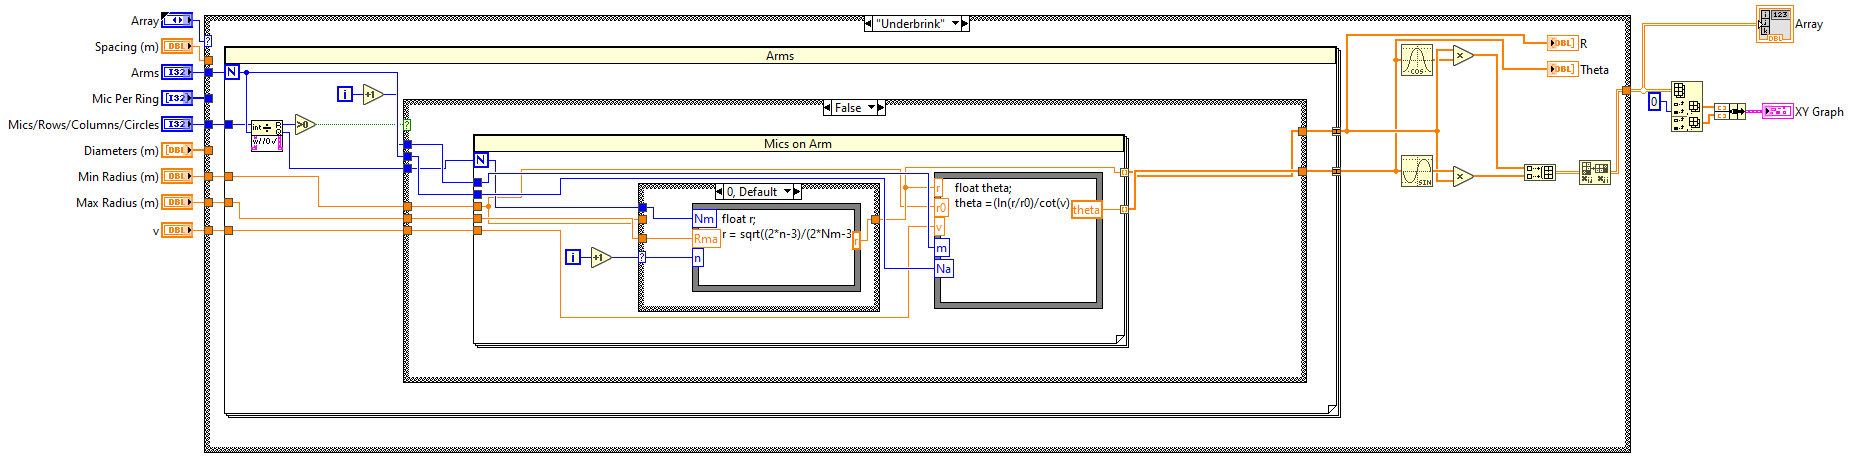
\includegraphics[keepaspectratio, width = \textwidth]{Figures/ArrayGenBlock.png}
        \caption{Array Generator LabVIEW Block Diagram}
        \label{fig:ArrayGenBlock}
    \end{figure}
    
    The LabVIEW block diagram only shows a partial snippet of the program and is the function for generating a custom under-brink array. Starting from the left, it takes the inputs of Arms, Minimum Radius, Maximum Radius and Arm Angle. These are processed through a math-script function block to calculate both the radius and angle of each particular microphone as according to the equations presented in Section \ref{sec:Array Geometry}, once processed the values are converted from cylindrical co-ordinates to Cartesian co-ordinates. On the right hand side of the diagram is the outputs, the XY graph that is shown in Figure \ref{fig:ArrayGenPanel} and the array of Cartesian co-ordinate.
    
    Below in Figure \ref{fig:ArrayGenPanel} the user interface for the Array Generator is shown. As well as giving various options for array customisation a live plot of the current array is displayed on the right hand side of the user interface.  
    
    \begin{figure}[H]
        \centering
        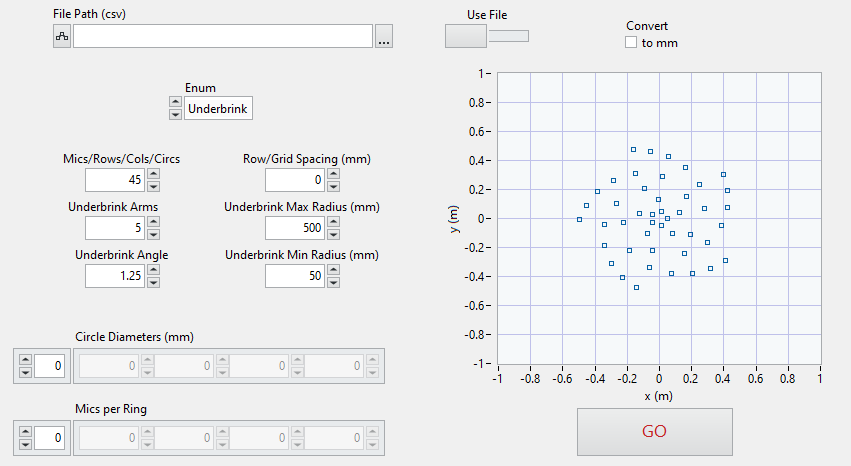
\includegraphics[keepaspectratio, width = 0.8\textwidth]{Figures/ArrayGenPanel.png}
        \caption{Array Generator LabVIEW Front Panel User Interface}
        \label{fig:ArrayGenPanel}
    \end{figure}
    
%%%%%%%%%%%%%%%%%%%%%%%%%%%%%%%%
\subsubsection{Delay Calculations} \label{sec:Delay Calculations}
    \hl{probably re write}
    At the core of all beamforming algorithms is the relative delays between each microphone for an impinging signal. This function shown in Figure \ref{fig:MicDelayBlock} applies Eqn. \ref{eq:TDOAx+y} and \ref{eq:TDOAfs}, by taking in the microphone array in Cartesian co-ordinates and generating an array of delays relative to the first microphone for a signal arriving at a particular Azimuth and Elevation.
    
    \begin{figure}[H]
        \centering
        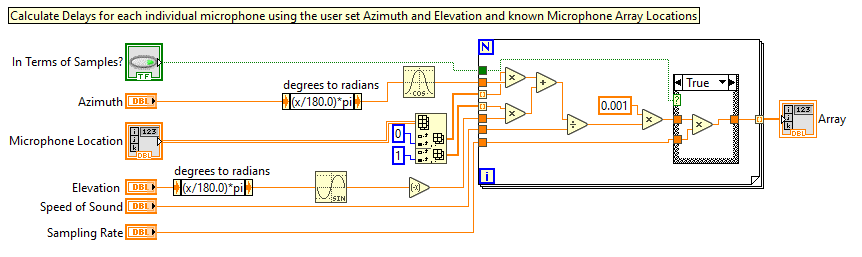
\includegraphics[keepaspectratio, width = \textwidth]{Figures/DelayCalcBlock.png}
        \caption{Microphone Relative Delay Generator LabVIEW Block Diagram}
        \label{fig:MicDelayBlock}
    \end{figure}    
    
    By iterating through this function for every single combination of Azimuth and Elevation a 3 dimensional array of delays is produced for, this includes the time or sample delay of every microphone for a signal coming from all possible combinations of Azimuth and Elevation in front of the microphone array. This function is at the core of all beamforming algorithms and simulations for recreating spatial signals.
    
%%%%%%%%%%%%%%%%%%%%%%%%%%%%%%%%
\subsubsection{Spatial Signal Generator} \label{sec:Signal Generator}
    Using the generated microphone array geometry and the generated array of microphone delays from Section \ref{sec:Array Generator} and \ref{sec:Delay Calculations} respectively equivalent spatial signals can be recreated for the purpose of simulating and testing microphone array performance. Figure \ref{fig:SignalGenBlock} shows the block diagram of the LabVIEW VI that performs the signal generation. This VI can recreate up to two separate spatial signals, with added white noise and has a choice of equivalent sampling rate and the number of samples capture. This allows for a more accurate representation of array performance and especially for the ratio of processing time to signal length and the effects of the signal length on algorithm and array performance. 
    
    \begin{figure}[H]
        \centering
        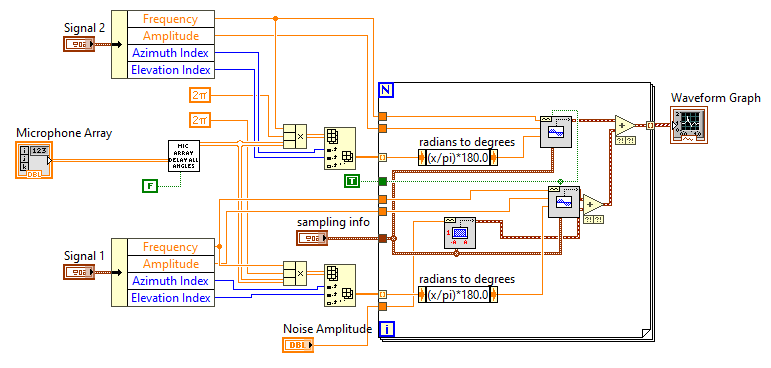
\includegraphics[keepaspectratio, width = \textwidth]{Figures/SignalGenBlock.png}
        \caption{Spatial Signal Generator LabVIEW Block Diagram}
        \label{fig:SignalGenBlock}
    \end{figure}    
    
    The spatial signals are simulated by calculating what the phase delay would theoretically be for a signal coming from a spatial location. For instance, to simulate a signal of frequency $f$ that is coming from a an azimuth of $\theta$ and elevation of $\phi$ the phase can be calculated using Equation \ref{eq:phase delay} by converting time in seconds to phase in degrees. The phase delay is calculated for each microphone to generate a separate signals for each to simulate the real world situation.
    
    \begin{equation}
        \tau_{\varphi} = \frac{\tau(\theta,\phi) \cdot f \cdot \pi}{180}
        \label{eq:phase delay}
    \end{equation}
    
    Figure \ref{fig:SignalGenPanel} shows the user interface for the spatial signal generator, besides giving a way to choose the values it has helped with algorithm development as it gives a way to visualise what perfectly delayed signals should look and therefore how the delay-and-sum algorithm works.
    
    \begin{figure}[H]
        \centering
        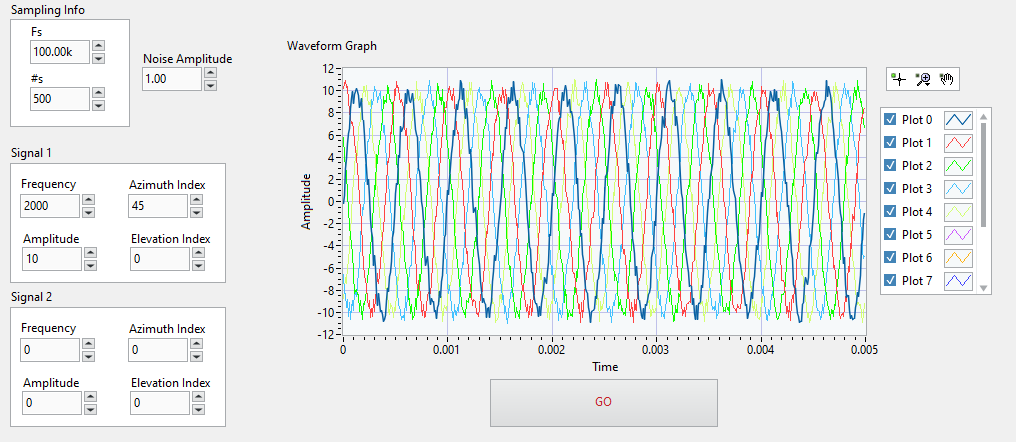
\includegraphics[keepaspectratio, width = 0.8\textwidth]{Figures/SignalGenPanel_5ULA50mm.png}
        \caption{Spatial Signal Generator LabVIEW Front Panel User Interface}
        \label{fig:SignalGenPanel}
    \end{figure}    

%%%%%%%%%%%%%%%%%%%%%%%%%%%%%%%%
\subsubsection{File Playback} \label{sec:File Playback}

The file playback function was added as a nice easy way to replay back data from testing and also gives the ability to choose any section of the file to perform beamforming with and perform post-processing.

Figure \ref{fig:FilePlaybackPanel} shows the user interface for playing back files, displaying the sound waves on the right and by zooming in on this plot different sections of the waveform can be used for processing.

    \begin{figure}[H]
        \centering
        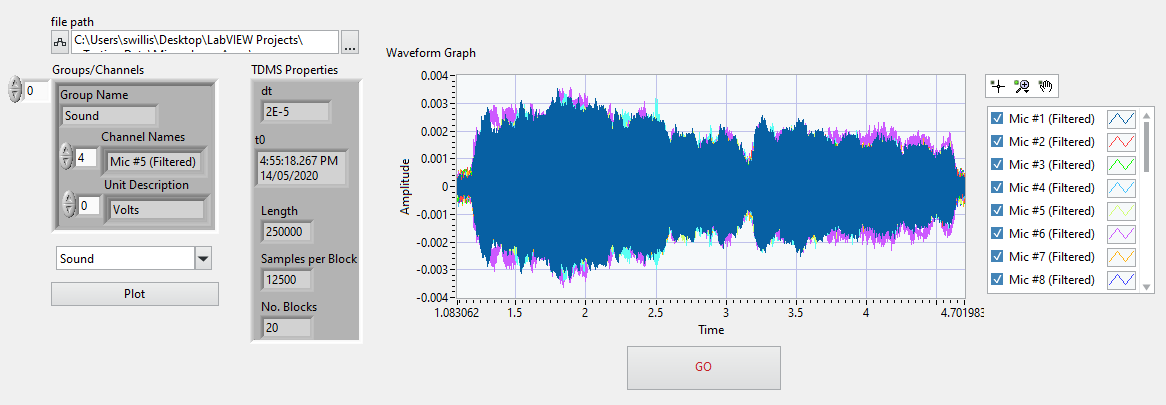
\includegraphics[keepaspectratio, width = 0.8\textwidth]{Figures/FilePlaybackPanel.png}
        \caption{File Playback LabVIEW Front Panel User Interface}
        \label{fig:FilePlaybackPanel}
    \end{figure}  

%%%%%%%%%%%%%%%%%%%%%%%%%%%%%%%%
\subsubsection{Simulation Testing and Validation} \label{sec:Sim Testing and Verification} 
    
    With the know known phase delay an array of sinusoidal waves are able to be generated with the correct phase that would theoretically be received at each sensor of the array. When this array of signals is input into any beamforming algorithm it ideally gives a performance gauge of the algorithm itself and the geometry of the array. When the output heat-map is compared against the 3D frequency response heat-map it is clear whether the results are as expected or not, Figure \ref{fig:Simulation Comparison} demonstrates this. The white is the estimated location of the signal source going down to blue then black as the least likely.
    
    \begin{figure} [H]
            \centering
            \begin{tabular}{ccc}
                \subfloat[Frequency Response]{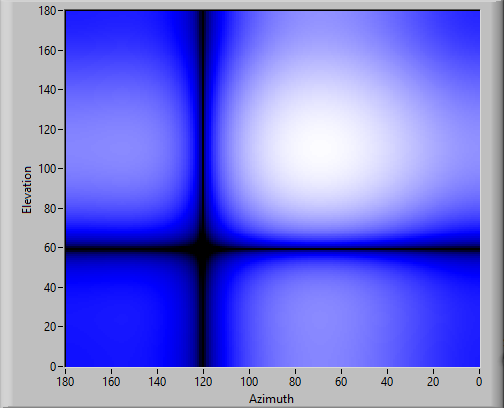
\includegraphics[keepaspectratio, width = 0.3\textwidth]{Figures/Sim3DResponse.png}} &
                \subfloat[Simulation Estimation]{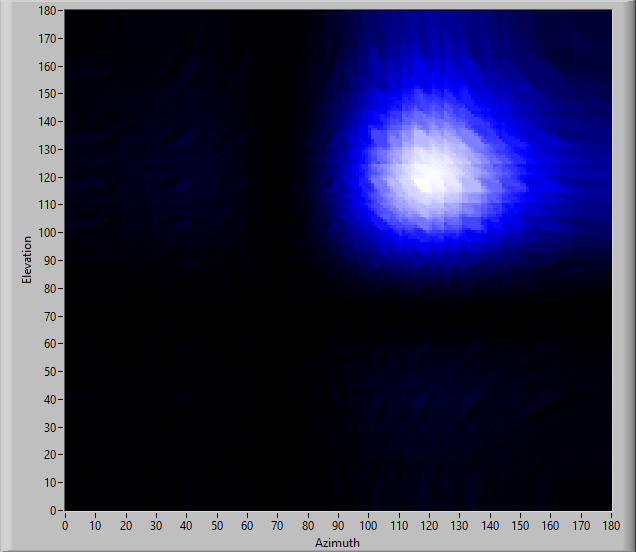
\includegraphics[keepaspectratio, height = 0.245\textwidth]{Figures/SimSignalHeatmap.png}} & 
                \subfloat[Frequency Response Main-lobe]{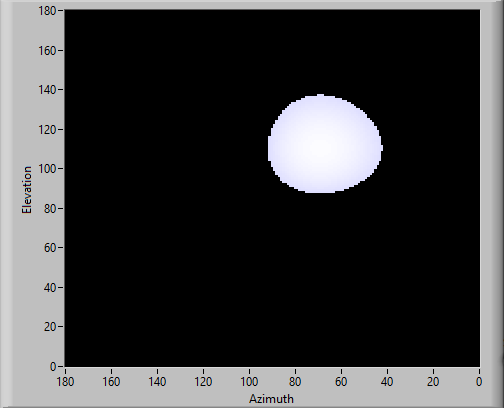
\includegraphics[keepaspectratio, width = 0.3\textwidth]{Figures/Sim3DResponseMainLobe.png}}\\
            \end{tabular}
            \caption{Comparison of Simulation Results to Expected Results}
            \label{fig:Simulation Comparison}
        \end{figure}
        
    Comparing the mathematical model used in the frequency response and the implemented delay-and-sum algorithm in the simulation both returned nearly the same results, this indicates that the delay-and-sum algorithm is working as intended and that the simulation works as intended as well. The two main side-lobs in Figure \ref{fig:Simulation Comparison}a can also be seen in Figure \ref{fig:Simulation Comparison}b towards the top left and bottom right for further verification. Additional Figures from this simulation are included in Appendix \ref{app:Sim} 
    
%%%%%%%%%%%%%%%%%%%%%%%%%%%%%%%%
\subsubsection{Algorithm Simulation Comparison} \label{sec:Algorithm Comparison}

    This section details the core differences found in simulating both the Delay-and-Sum Algorithm and the MUSIC Algorithm. Figure \ref{fig:Alg Comp Single} shows the comparison of the two algorithms response to a single 1863Hz frequency signal at 13 Degrees to the left of centre Azimuth and 16 Degrees below the centre Elevation.
    
    \begin{figure} [H]
        \centering
        \begin{tabular}{cc}
            \subfloat[Delay and Sum Algorithm]{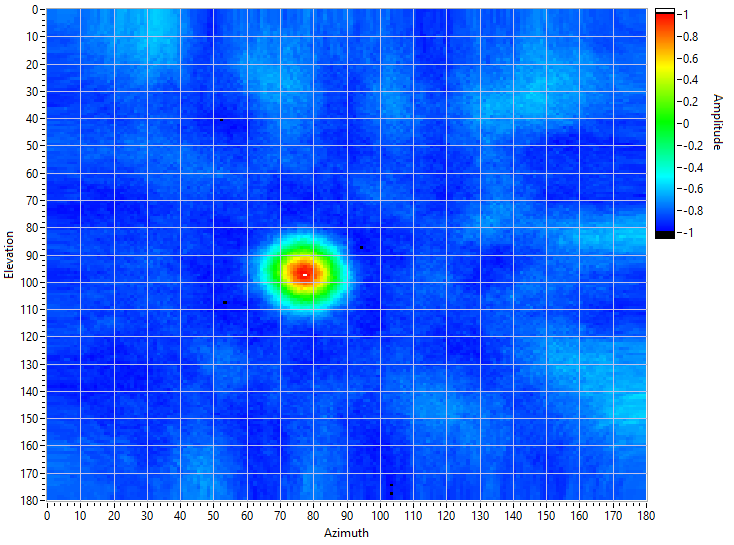
\includegraphics[keepaspectratio, width = 0.4\textwidth]{Figures/Az13_El6_DAS_SIM_01s.png}} &
            \subfloat[MUSIC Algorithm]{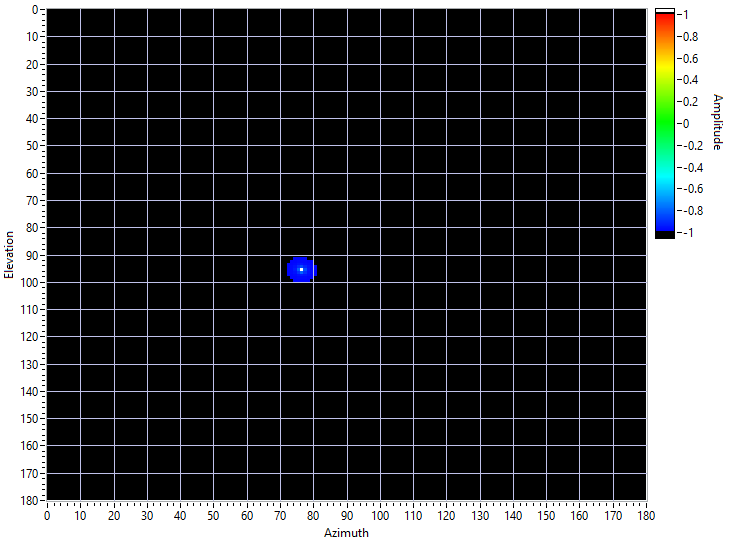
\includegraphics[keepaspectratio, width = 0.4\textwidth]{Figures/Az13_El6_MUSIC_Sim_8s.png}}
        \end{tabular}
        \caption{DAS and MUSIC Algorithms compared at 1863Hz}
        \label{fig:Alg Comp Single}
    \end{figure}
    
    The differences between algorithms is very clear. To make the comparison as fair as possible the input signals were of different lengths to make the compute time equal which starts to show the computational differences between the two. The input signals for MUSIC was 8 seconds long while the input signals for delay-and-sum were 0.1 seconds. MUSIC algorithm outperforms the delay-and-sum drastically, as it estimates the signal location to pin-point accuracy, the delay-and-sum's most likely estimation is only a few degrees off the real location, though looking at the estimation results it could realistically be anywhere within the 7 degree radius hot-spot.
    
    Figure \ref{fig:Alg Comp Blind} shows a test of the ability of both algorithms to separate two signals of the exact same frequency. Two single frequency 1863Hz signals were produced both on the horizontal and 12 Degrees either side of the centre giving 24 Degrees of separation, 24 degrees was chosen as it was the smallest degree of separation that both algorithm could separate the signals. The same length of input signals was used as the previous example to keep it comparable. This test shows slightly different results but still the MUSIC algorithm performs better as it has a definite differentiation between the signals but the estimation of location of the left signal is not correct, whilst the delay-and-sum has only just differentiated the signals but is giving a broader area of location estimations.

    \begin{figure} [H]
        \centering
        \begin{tabular}{cc}
            \subfloat[Delay and Sum Algorithm]{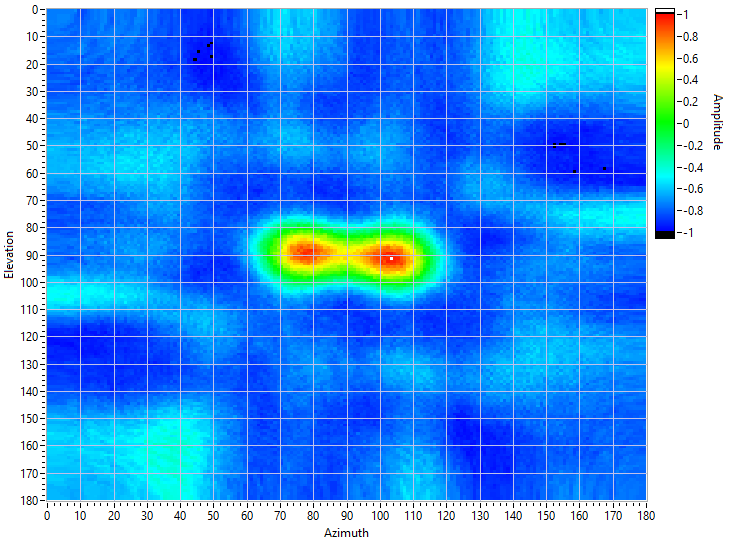
\includegraphics[keepaspectratio, width = 0.4\textwidth]{Figures/24Deg_1863_DAS.png}} &
            \subfloat[MUSIC Algorithm]{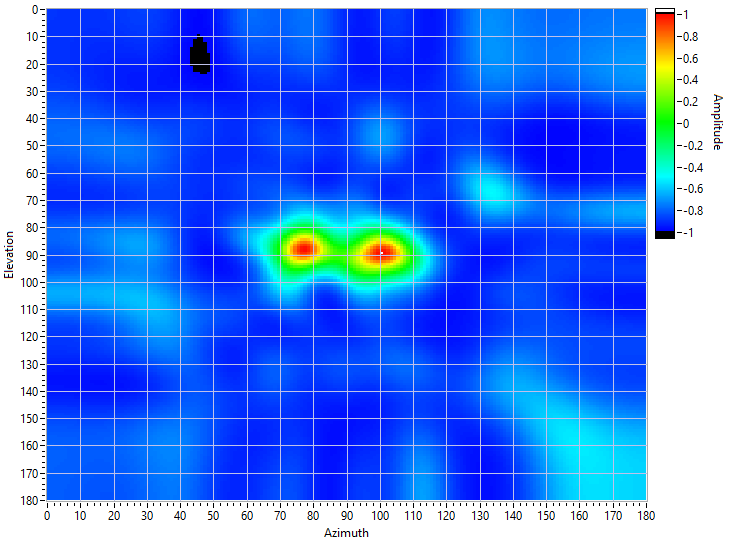
\includegraphics[keepaspectratio, width = 0.4\textwidth]{Figures/24Deg_1863Hz_MUSIC.png}}
        \end{tabular}
        \caption{DAS and MUSIC Algorithms compared at 1863Hz Source Separation}
        \label{fig:Alg Comp Blind}
    \end{figure}
    
    Overall through extensive testing it was found that the delay-and-sum algorithm was a much more robust algorithm but is essentially attempting to find the strongest sound source in its view which can lead to misleading results, as well as this it is much more computationally intensive compared to the MUSIC algorithm. The MUSIC algorithm performed significantly better and quicker than the delay-and-sum algorithm in simulation showing great potential but does require more knowledge of the signal of interest for it to be effective as well as fast.
    
%%%%%%%%%%%%%%%%%%%%%%%%%%%%%%%%
\newpage
\section{Hardware Research and Development} \label{sec:Hardware}
%%%%%%%%%%%%%%%%%%%%%%%%%%%%%%%%
\subsection{2D Frequency Response} \label{sec:2D Freq Response}
    A Frequency response is a visual way of analysing the effectiveness of microphone array geometries to a certain frequency coming from particular directions and allows for a quick analysis of array geometries. A frequency response for a uniform linear array of 10 microphones with a spacing of $8$cm subject to a 2kHz signal is pictured in Figure \ref{fig:2DFreqResponseLin} and the same response when digitally steered to 130$^{\circ}$ in Figure \ref{fig:2DResponseSteered}.
    
    \begin{figure}[H]
        \centering
        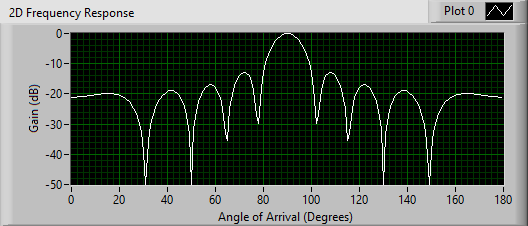
\includegraphics[keepaspectratio, width = 0.6\textwidth]{Figures/FrequencyResponse2K10Lin.png}
        \caption{2D Frequency Response}
        \label{fig:2DFreqResponseLin}
    \end{figure}
    \begin{figure}[H]
        \centering
        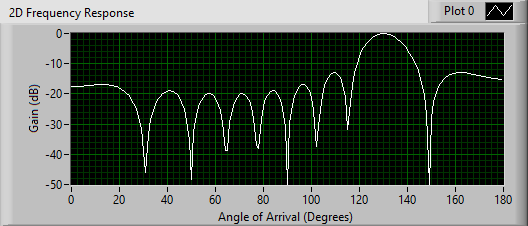
\includegraphics[keepaspectratio, width = 0.6\textwidth]{Figures/2DResponseSteered.png}
        \caption{2D Frequency Response Steered to 130$^{\circ}$}
        \label{fig:2DResponseSteered}
    \end{figure}
    
    When evaluating a 2D Frequency response the main points of interest are the main-lobe, its beam-width and the side-lobes. The main-lobe is the lobe with the greatest amplitude seen at 90$^{\circ}$ in Figure \ref{fig:2DFreqResponseLin} the beam-width is the width from where the main-lobe drops to -20dB as this is half the power of 0dB, this is effectively the resolution of the array at that frequency. side-lobes are important to show the effective gain of interference that appear to be coming from angles other than the angle of interest due to spatial aliasing, these can be seen in Figure \ref{fig:2DFreqResponseLin} and \ref{fig:2DResponseSteered} by the 7 or 8 lobes with peaks around -20dB gain. The goal of microphone array geometry design is to minimise the side-lobes minimizing interference, and decreasing the beam width to give a better array resolution.
    
    Equation \ref{eq:2D Response} was adapted from \citet{Ben08} and has been applied to calculate 2D Frequency responses in Figures \ref{fig:2DFreqResponseLin} and \ref{fig:2DResponseSteered}.
    
    \begin{equation}
        Response(\theta) = 20log_{10} \Big( \Big|\frac{\sum_{n=1}^N exp(\frac{-2\pi jx_n(cos(\theta)-cos(\varphi))}{c})}{N}\Big| \Big)
        \label{eq:2D Response}
    \end{equation}
    
    $\theta$ defined as the angle of arrival, where $x$ is the location in the $x$-direction from the origin, and $\varphi$ is the steered angle of the beamformer.
    
    Another useful visualisation using Equation \ref{eq:2D Response} is a form of Frequency response that repeats the 2D Frequency response above over a range of frequencies, this makes it easier to spot if there are any problem frequencies due to the array geometry. Using the same array as Figure \ref{fig:2DFreqResponseLin}, Figure \ref{fig:2DVaryFreqResp} shows the frequency response from $0$Hz to $6$kHz.
    
    \begin{figure}[H]
        \centering
        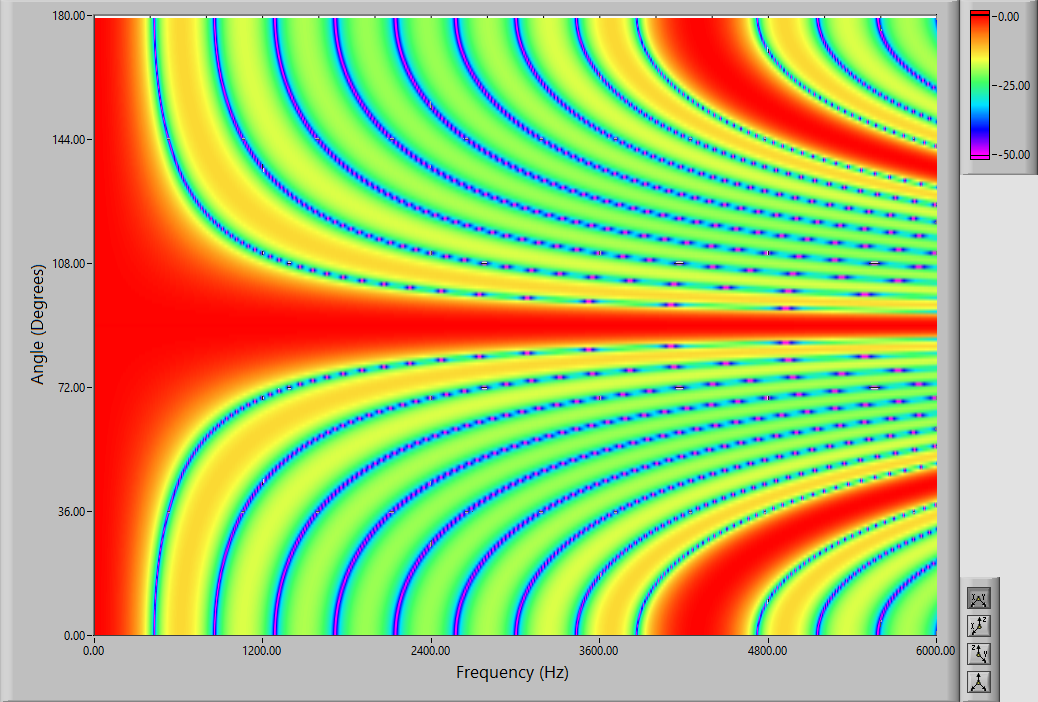
\includegraphics[keepaspectratio, width = 0.8\textwidth]{Figures/2DVaryFreqResp.png}
        \caption{2D Frequency Response over Varying Frequencies}
        \label{fig:2DVaryFreqResp}
    \end{figure}
    
    Figure \ref{fig:2DVaryFreqResp} demonstrates precisely how useful it can be for spotting problem frequencies for particular array geometries. We can see at around $4$kHz another main-lobe begins, this will make it impossible to determine where the signal is truly coming from as it would seem as it is coming from 3 directions this is due to the microphone array sensor spacing being a multiple of the signal wavelength causing spatial aliasing to occur, creating misleading results. As can be calculated with Equation \ref{eq:wavelength} just below 4kHz the wavelength is 8cm, exactly the same as the microphone spacing, providing reason for the spatial aliasing.
    
    Another important property of this array is where it becomes use-able, before $400$Hz the array has no directionality and cannot determine the direction of a source of interest. The lack of directionality is due to the aperture of the array as mentioned in Section \ref{sec:Signal Processing}, below $400$Hz the signal wavelength is larger than the array aperture hence it is useless for directionality below this point.
    
    2D Frequency Response analysis of microphone arrays is useful if the geometry of the array is symmetrical. The 2D Response is only looking at the angle of arrival across one of the axes, in this case the angle of arrival is moving across the array azimuth and therefore we cannot see the response of a signal moving through the elevation. For arrays that are symmetrical this doesn't matter as the response will be the same for both azimuth and elevation. A more useful analysis for non-symmetrical array geometry is 3D Frequency Response.
%%%%%%%%%%%%%%%%%%%%%%%%%%%%%%%% 
\subsection{3D Frequency Response} \label{sec:3D Freq Response}
    3D Frequency response is based on Equation \ref{eq:3D Response} using a modified version of Equation \ref{eq:2D Response}, adding a way to analyse the $y$ location of each microphone and its respective response due to that.
    
    \begin{equation}
        Response(\theta) = 20log_{10} \Big( \Big|\frac{\sum_{n=1}^N exp(\frac{-2\pi j(x_n(cos(\theta)-cos(\varphi_A))+y_n(sin(\phi)-sin(\varphi_E))}{c}))}{N}\Big| \Big)
        \label{eq:3D Response}
    \end{equation}
    
    The main difference between the equation for 2D and 3D Frequency Response is the added factor for the steering and response along the elevation so a response can be found for all spatial locations in front of the array. Figure \ref{fig:3D Responses}(a), \ref{fig:3D Responses}(b), \ref{fig:3D Heatmap} and are the results for a 3D Frequency response for a grid array with 16 Microphones, 4 rows, 4 columns with a row and column spacing of 8cm subject to a 2kHz signal and digitally steered towards the origin of the array.

    \begin{figure} [H]
        \centering
        \begin{tabular}{cc}
            \subfloat[3D Frequency Response in Decibel]{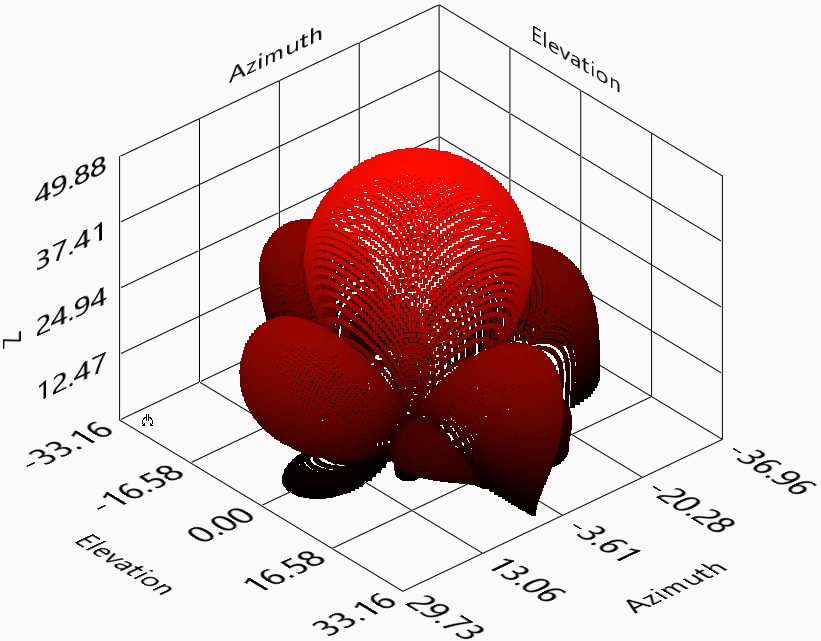
\includegraphics[keepaspectratio, width = 0.45\textwidth]{Figures/3DdBFigure.png}} &
            \subfloat[3D Frequency Response Linear Scale]{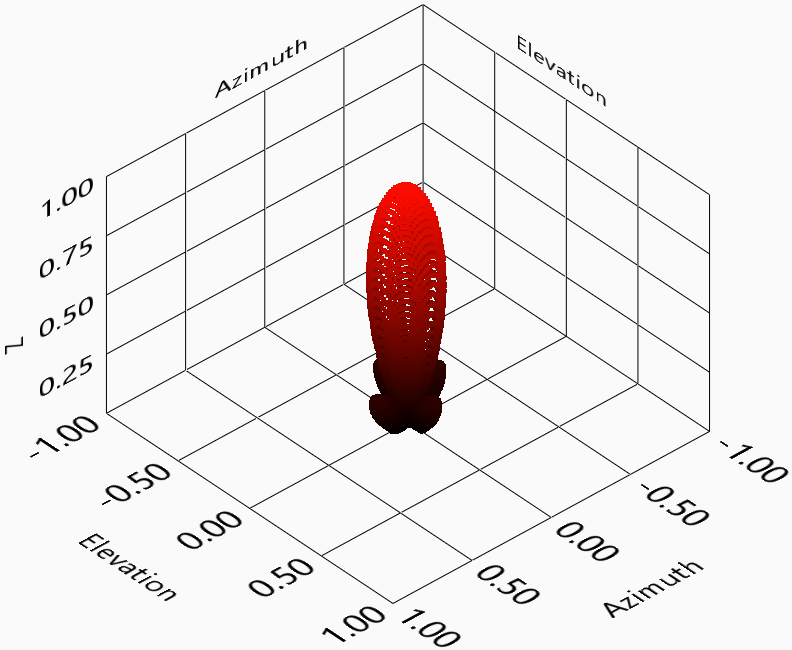
\includegraphics[keepaspectratio, width = 0.45\textwidth]{Figures/3DLinearFigure.png}}
        \end{tabular}
        \caption{3D Frequency Responses}
        \label{fig:3D Responses}
    \end{figure}
    
    Figure \ref{fig:3D Responses}(a) and \ref{fig:3D Responses}(b) are both 3D Frequency Responses from the same array with different scaling, the decibel scaling can be useful for a lot of analysis as it attenuates the side-lobes a lot more than a linear scale. These figures allow easy visualisation of the side-lobes and nulls that appear at any particular frequency, these are just a 3D representation of the heat-map in Figure \ref{fig:3D Heatmap}, the heat-map is the most useful for visualising array performance due to the ease of interpretation.
    
    \begin{figure}[H]
        \centering
        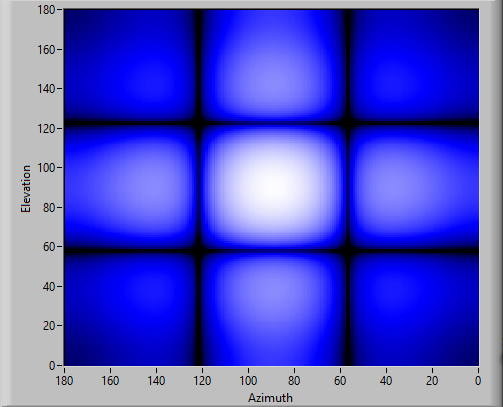
\includegraphics[keepaspectratio, width = 0.6\textwidth]{Figures/3DHeatFigure.png}
        \caption{3D Frequency Response Heatmap in Decibel}
        \label{fig:3D Heatmap}
    \end{figure}
    
    When analysing an array geometry using a heat-map like the one pictured in Figure \ref{fig:3D Heatmap} the high points are in white going through blue to black at the lowest. This grid array in particular has 1 main-lobe pictured in the centre as the white area and 4 particularly high side-lobes on all sides of the main-lobe with nulls in between. This array shows a good response at this frequency but at different frequencies it is clear it will experience spatial aliasing with such prominent side-lobes. These side-lobes can also be clearly seen in Figure \ref{eq:3D Response}(a). The one drawback of the 3D Frequency response is only being able to analyse a single frequency at a time.

%%%%%%%%%%%%%%%%%%%%%%%%%%%%%%%%
\subsection{Geometry Design} \label{sec:Array Geometry}

    The main constraints with the design of microphone array is the number of handle-able synchronised high sample-rate analog inputs.
    
    A comparison of various array geometries was performed by Zebb Prime and Con Doolan of The University of Adelaide, this included various spiral array geometries that were evaluated by comparing their minimum side-lobe levels and beam widths. A comparison of all the arrays for both near-field and far-field was presented but as the purpose of the array in this report is for far-field signals the near field results were not taken into account. The comparison showed the the Underbrink geometry design was overall the best performing closely followed by the Brüel \& Kjær (B\&K) array \citep{Pri13}. Hence for the choice of array for the proof of concept design the Underbrink array was chosen as it shows promising resolution and minimal side-lobes especially for the number of sensors being used.
    
    The Underbrink array is shown in Figure \ref{fig:Mic Arrays}, it is a "multi-spiral design where the microphones are placed in the centre of equal area segments" \citep{Pri13}. Where a minimum and maximum radius ($r_0$ and $r_{max}$ respectively) must be defined as well as the number of spiral arms ($N_a$) and microphones per spiral ($N_m$). This array is based upon the following set of equations.
    
    The radius of each individual microphone:
    \begin{equation}
        r_{m,1} = r_0,\;\;m=1,...,N_a
    \end{equation}
    \begin{equation*}
        r_{m,n}=\sqrt{\frac{2n-3}{2N_r-3}}r_{max},\;\;m=1,...,N_a\;\;n=2,...,N_m
    \end{equation*}
    The angle of each individual microphone:
    \begin{equation}
        \theta_{m,n} = \frac{ln(\frac{r_{m,n}}{r_0})}{cot(v)} + \frac{m-1}{N_a}2\pi,\;\;m=1,....N_a,\;\;n=1,...,N_m
    \end{equation}
    \begin{equation*}
        where,\;\;v=\frac{5\pi}{16}
    \end{equation*}
    
    To be able to generate many different configurations of the Underbrink array a Python script was initially written, this script also converted the coordinates from polar to Cartesian making it easier to work with the LabVIEW Simulations. As progression was made with LabVIEW this was converted to a LabVIEW module for better integration to the full simulation package. 
%%%%%%%%%%%%%%%%%%%%%%%%%%%%%%%%
\subsubsection{First Design} \label{sec:First Array Design}
    For the initial testing of microphone arrays and verification that it would be possible the available hardware I designed an Underbrink array with an inner radius of 25mm and outer radius of 250mm, 3 arms with 4 microphones each. The reason for 12 microphones was due to a hardware limit as there were only 12 available high speed analog input cards for data acquisition at the time. Through the initial design process it was found that the Underbrink array performed better when there was an odd number of arms as it prevent the array from being symmetrical and significantly reduced the side-lobe levels and spatial aliasing as is further investigated in Section \ref{sec:Second Array Design}, a scatter plot of the designed array is pictured in \ref{fig:Testing Array}.
    
    \begin{figure} [H]
        \centering
        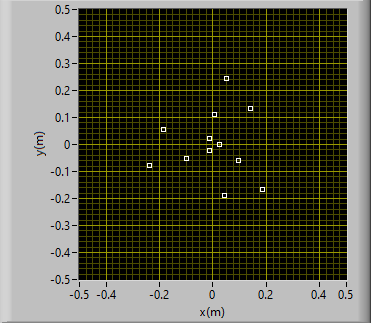
\includegraphics[keepaspectratio, width = 0.6\textwidth]{Figures/CurrentTestingArray.png}
        \caption{Chosen Underbrink Array}
        \label{fig:Testing Array}
    \end{figure}
    
    The choice of the inner and outer radius dimensions were based off of the frequency response and ease-of-building, giving very minimal side-lobe levels and a acceptable resolution between 1kHz and 4.5kHz without being overly large. Designs were considered with larger radii to have a better response at lower frequencies but for the current purpose of testing algorithms and whether the microphone array will actually work the frequency range is not a problem.
    
    Figure \ref{fig:Underbrink Response}(a) and \ref{fig:Underbrink Response}(b) show the frequency response for this custom Underbrink array at 2kHz, compared to the grid array shown in Section \ref{sec:2D Freq Response} the Underbrink shows very minimal side-lobe levels or obvious side-lobes and no spatial aliasing giving a promising response for the amount of sensors hence the choice for further testing.  

    \begin{figure} [H]
        \centering
        \begin{tabular}{cc}
            \subfloat[Underbrink Array 3D Response in Decibel]{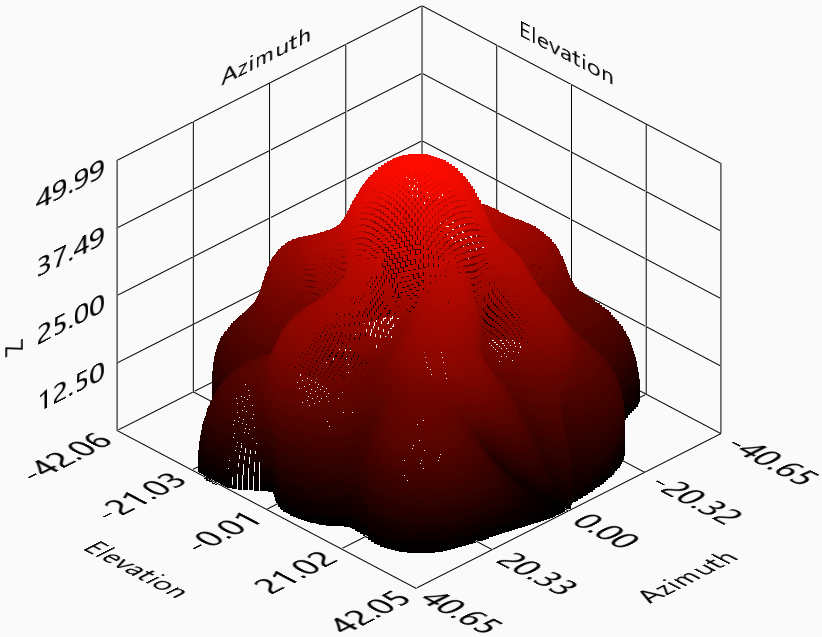
\includegraphics[keepaspectratio, width = 0.45\textwidth]{Figures/3DdB12mm.png}} &
            \subfloat[Underbrink Array 3D Response Heatmap]{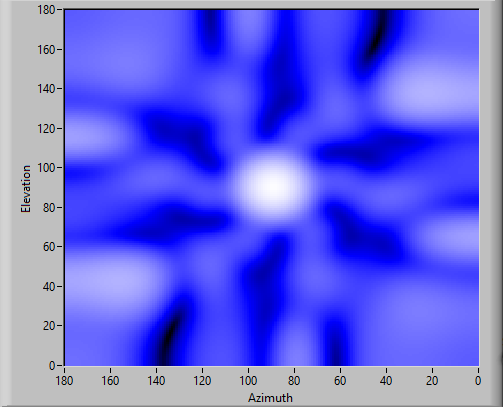
\includegraphics[keepaspectratio, width = 0.45\textwidth]{Figures/3DHeat12mm.png}}
        \end{tabular}
        \caption{Underbrink Array 3D Responses}
        \label{fig:Underbrink Response}
    \end{figure}
    
    Below Figure \ref{fig:TestArray} shows the array that was used in this first design, this was constructed from a sheet of cardboard as this allowed for easy prototyping of an array of this size, holes were cut at the exact location of the microphones which allowed for easy mounting with a screw and an additional hole made for the cables to be run through. The main problem with a design like this is the potential for reverberation noise from the solid back-plane of the array.
    
    \begin{figure} [H]
        \centering
        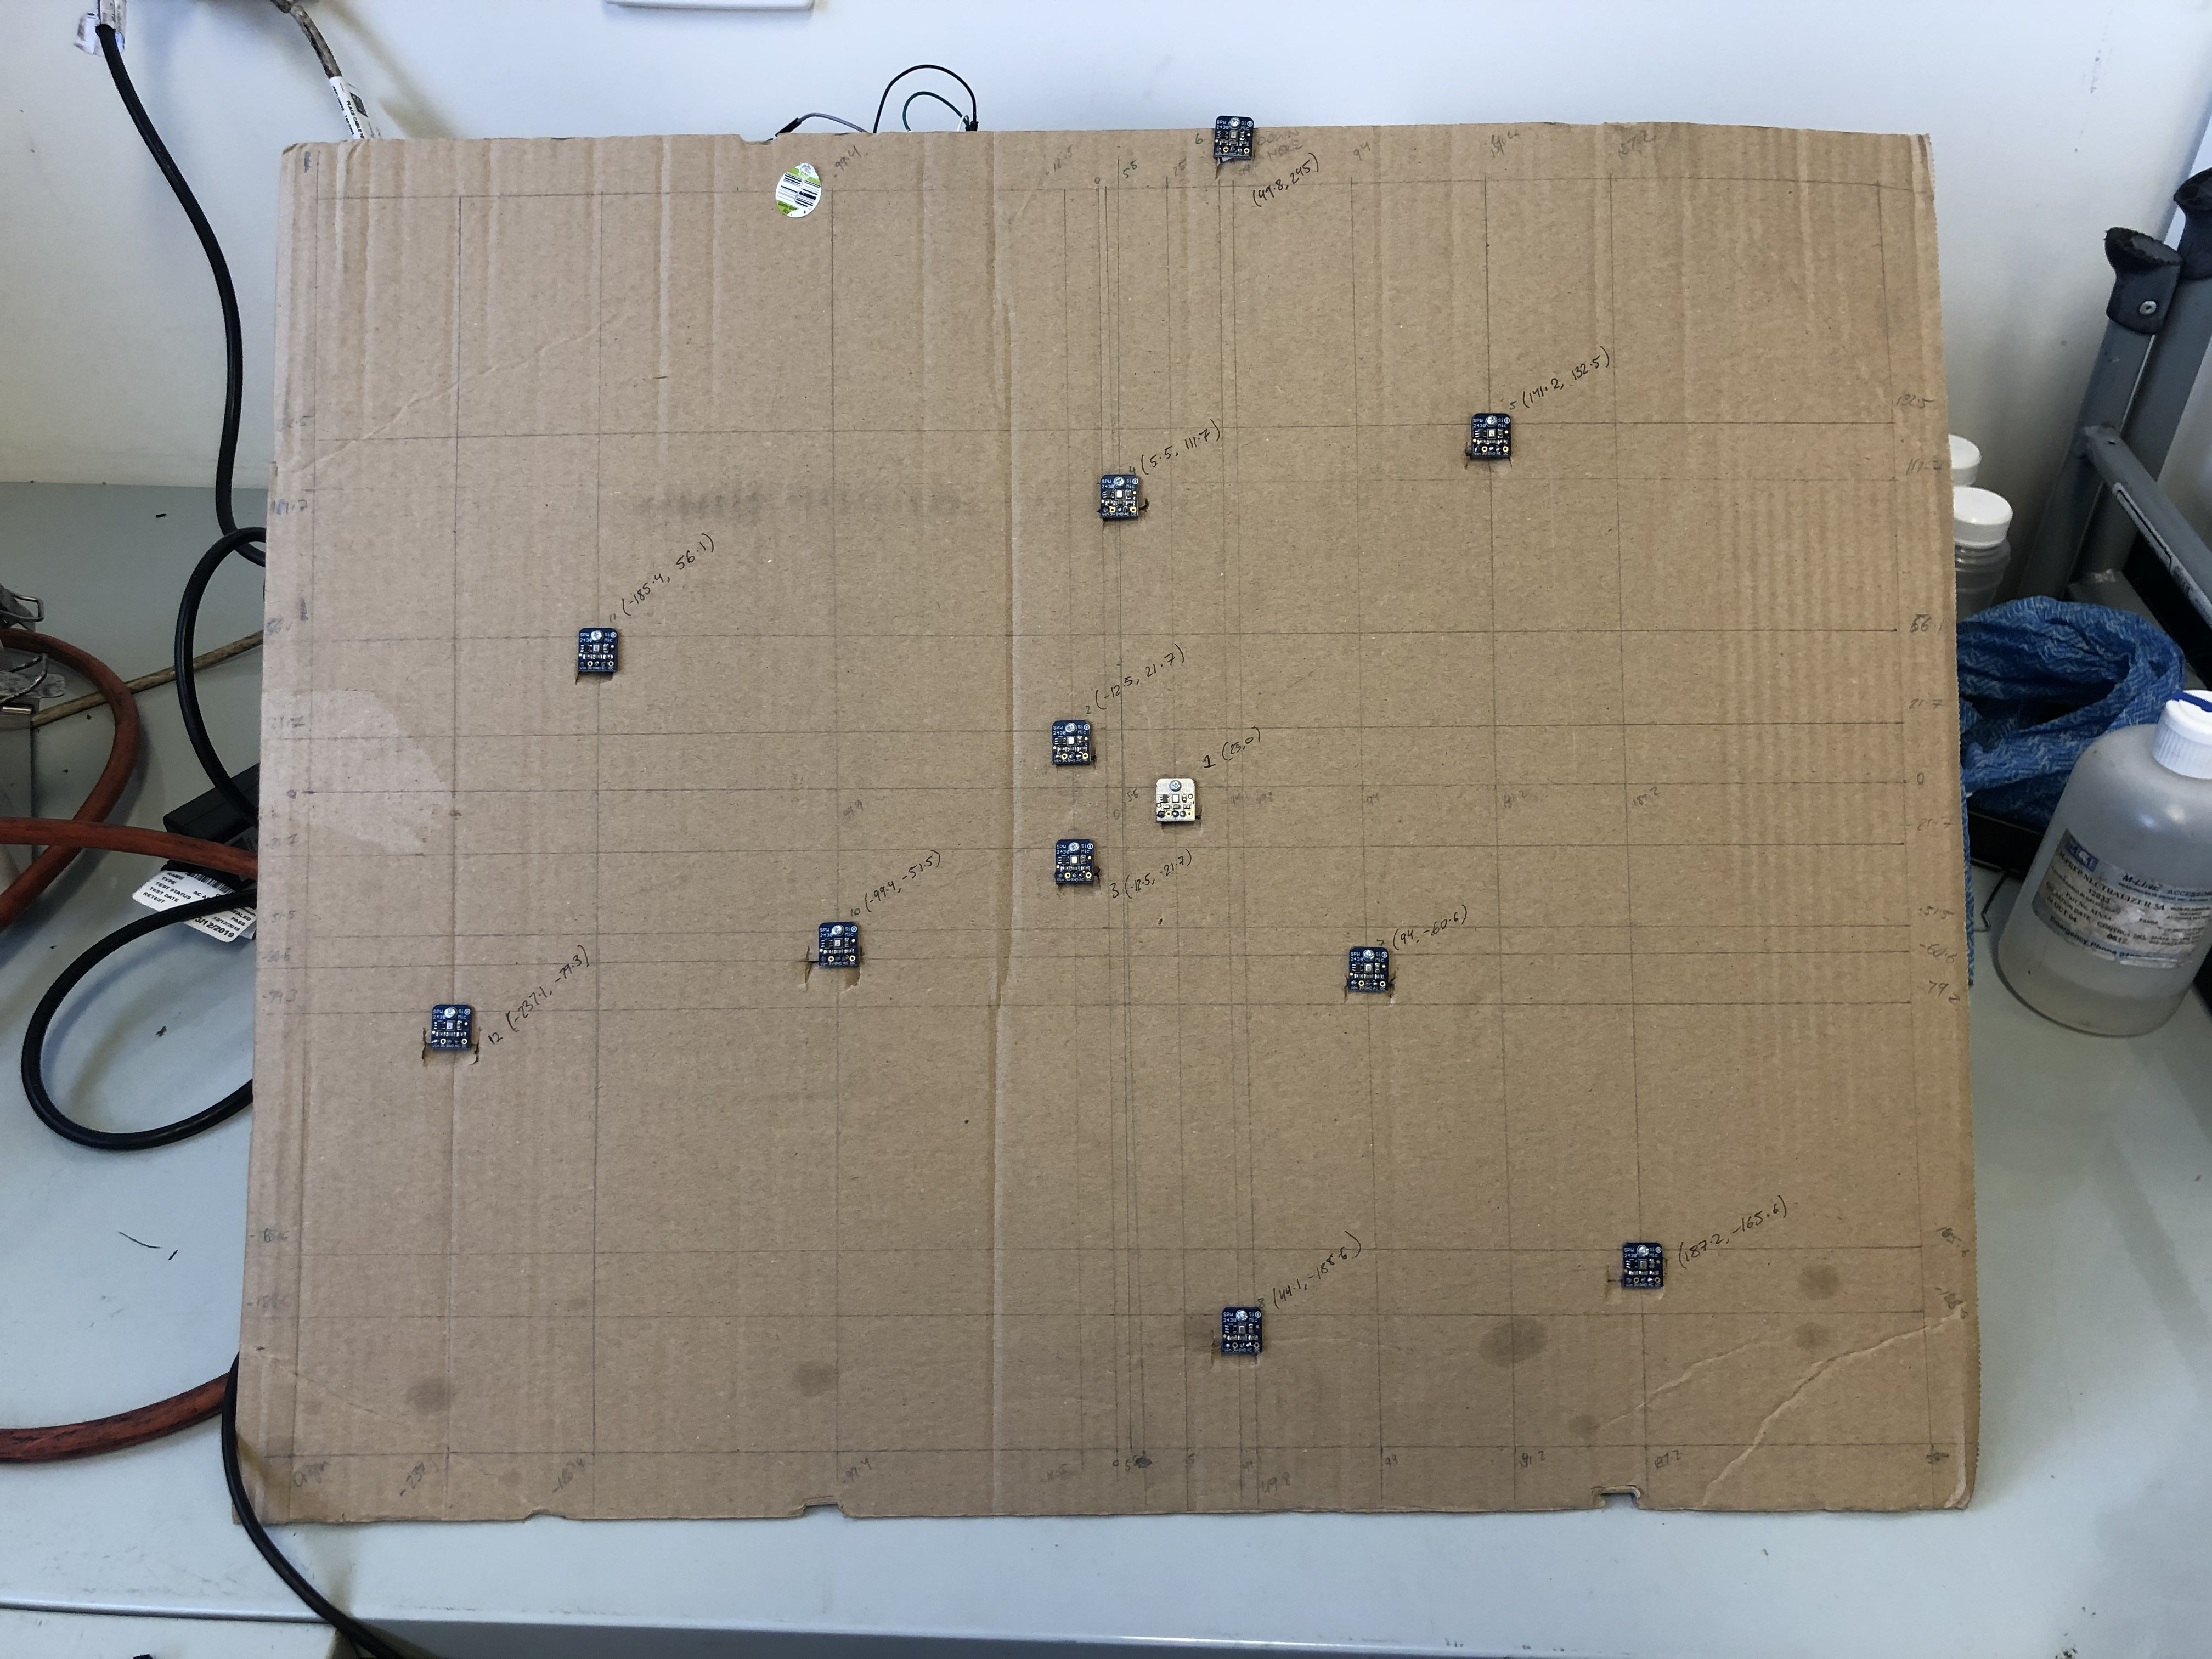
\includegraphics[keepaspectratio, width = 0.6\textwidth]{Figures/CardboardArray.jpeg}
        \caption{Initial Microphone Array}
        \label{fig:TestArray}
    \end{figure}
    
%%%%%%%%%%%%%%%%%%%%%%%%%%%%%%%%
\subsubsection{Second Design} \label{sec:Second Array Design}
    For the second iteration of the microphone array my limit was increased to 48 synchronous analog channels. This was to be achieved using two separate National Instrument cRIO-9036's both filled with 8 NI-9232's capable of 3 analog channels sampling at 102.4kHz.
    
    The Figures for this section can be found in Appendix \ref{app:Geom Invest}.
    
    Through an investigation of Underbrink array designs found that an odd number of arms performs better than an even number when using a similar number of microphones. This is found to be due to the symmetrical geometry produced by an even number of arms that causes the problem of spatial aliasing. The series of microphone array geometries used to demonstrate this is displayed in Appendix \ref{app:Geometries}, these geometries range from 42 to 48 microphones being used from 5 to 9 arms and all with a minimum radius of 25mm and maximum radius of 0.5m as this gave the best possible frequency response without the array becoming too large to easily move, carry and transport. The theoretical frequency response of an array of this size will be from 686Hz to beyond the 10kHz limit of the microphones.
    
    Appendix \ref{app:frequencies} features the 3D Frequency Response of each of the arrays from Appendix \ref{app:Geometries} when subject to a pure 4kHz signal at the absolute centre of the array. This demonstrates that purely having a great number of microphones will not result in a better performing array and that other choices made with the geometry will see better improvements in performance. All of the geometries have a near identical beam-width, this was expected as the used 4kHz signal is well within all of their ideal frequency response range, and with all of the arrays having equal inner and outer radius' no array should have an advantage. Both microphone arrays utilising the full 48 microphones show significantly larger side-lobe levels than the arrays with less microphones due to the even number of arms on the array.
    
    Taking into consideration the results of the various array geometries the geometry shown in Appendix \ref{app:Geometries}(a) with 5 arms was chosen for the new array design, this was due to two reason; firstly the array showed similar side-lobe levels to the 7 arm and 9 arm geometries but had fewer side-lobes, secondly with a desired inner radius of 25mm it would not be possible to fit more than 5 microphones easily. This design can also be seen in the finished design shown in Figure \ref{fig:Final Array}.
        
    Now with the desired design chosen further analysis was performed to ensure adequate performance from the array. Using the same technique shown in Section \ref{sec:2D Freq Response} producing a series of 2D Frequency responses through all the use-able frequencies to see a more accurate representation of the array response.  This was performed for both the 2D response of the Azimuth and Elevation as a 3D frequency response is just a combination of these, performing them separately provides similar results but the ability to see the response over the desired frequencies. Figure \ref{fig:Final Az Beam Pattern} shows the frequency response across the azimuth of the array ranging from 0 to 10kHz and Figure \ref{fig:Final El Beam Pattern} showing the same frequency range across the elevation of the array.
        
        \begin{figure} [H]
        \centering
        \begin{tabular}{cc}
            \subfloat[Final Array Azimuth Zoomed Beam Pattern]{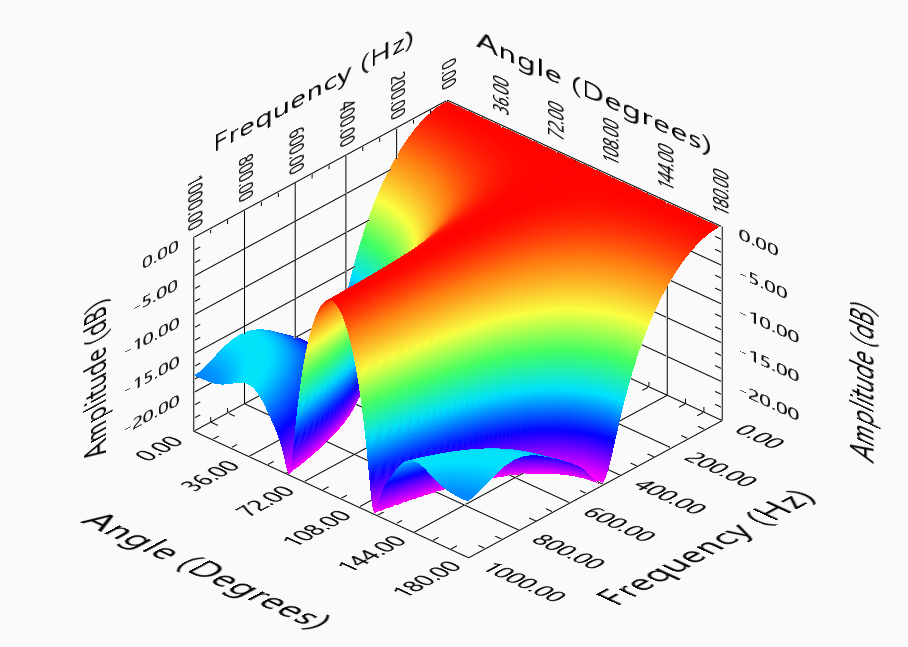
\includegraphics[keepaspectratio, width = 0.45\textwidth]{Figures/FinalAzLowBeamPAttern.png}} &
            \subfloat[Final Array Azimuth Full Beam Pattern]{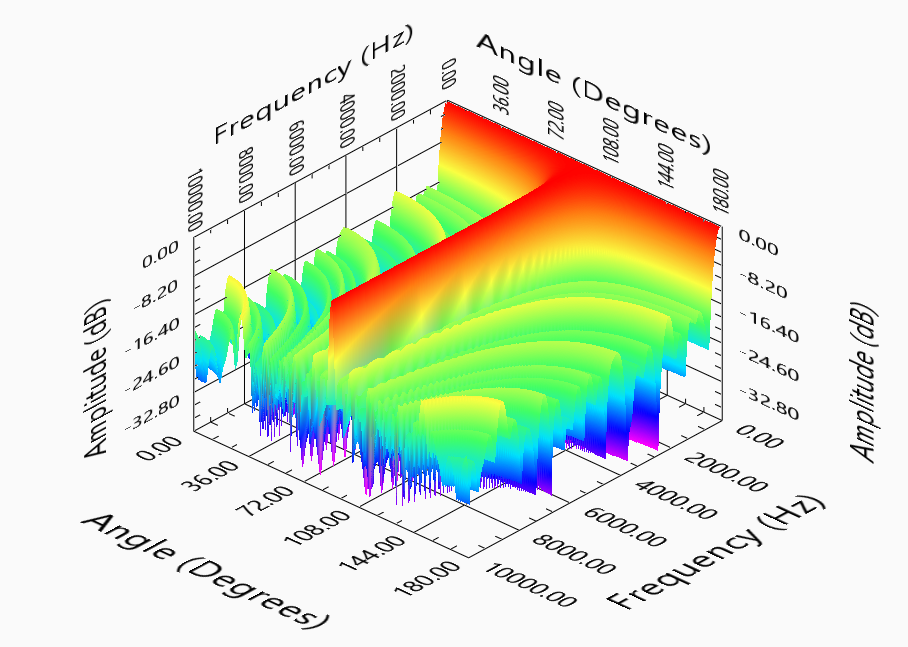
\includegraphics[keepaspectratio, width = 0.45\textwidth]{Figures/FinalAzBeamPatter.png}}
        \end{tabular}
        \caption{Final Array Azimuth Frequency Sweep Beam Patterns}
        \label{fig:Final Az Beam Pattern}
        \end{figure}
        
        \begin{figure} [H]
        \centering
        \begin{tabular}{cc}
            \subfloat[Final Array Elevation Zoomed Beam Pattern]{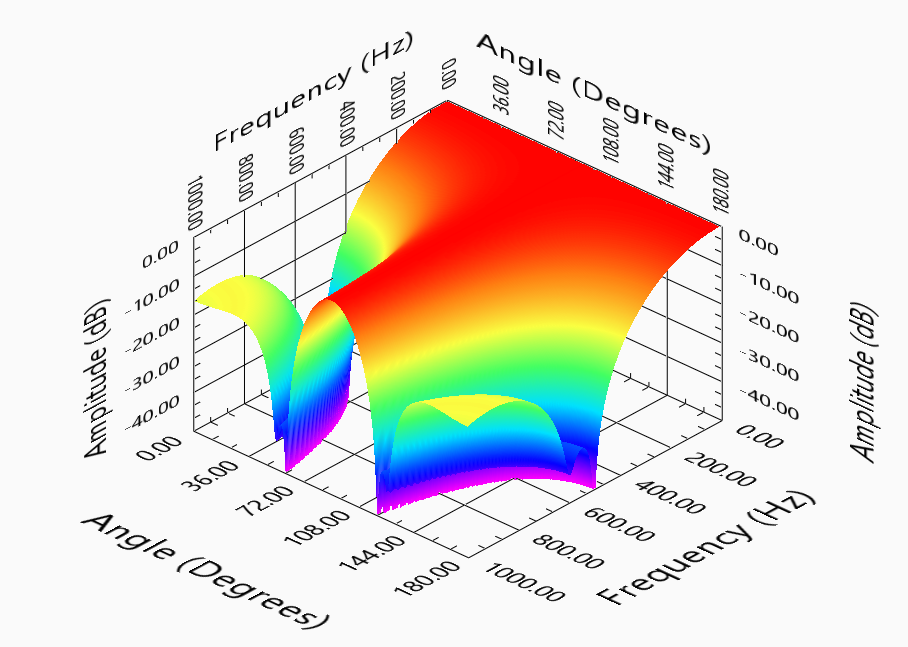
\includegraphics[keepaspectratio, width = 0.45\textwidth]{Figures/FinalElLowBeamPattern.png}} &
            \subfloat[Final Array Elevation Beam Pattern]{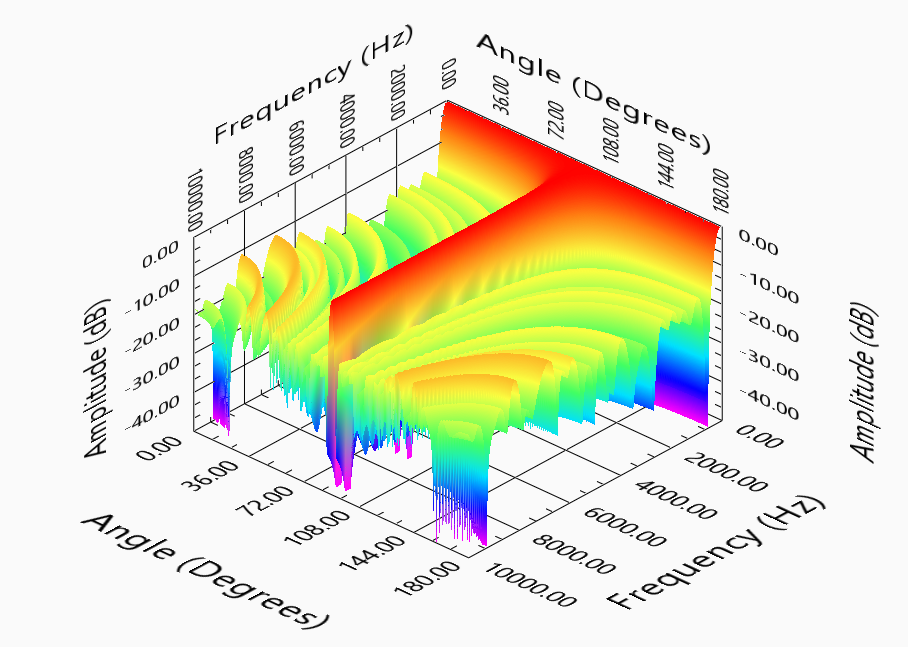
\includegraphics[keepaspectratio, width = 0.45\textwidth]{Figures/FinalElBeamPattern.png}}
        \end{tabular}
        \caption{Final Array Elevation Frequency Sweep Beam Patterns}
        \label{fig:Final El Beam Pattern}
        \end{figure}
        
    As shown in both of the sweeping 2D frequency responses' the array has very minimal side-lobe levels from 600Hz through to 10kHz. The array begins to have directionality around 750Hz due to the array diameter. Following Eqn. \ref{eq: aperture calc} with the array diameter of 1m it would equate to 686Hz as can be verified when looking at the frequency response. This relationship is due to spatial aliasing and the requirement for their two be two sensors within the wavelength of the signal as described in Section \ref{sec:Signal Processing}.
        
        \begin{equation}
            dia. > \frac{2c}{f}
            \label{eq: aperture calc}
        \end{equation}
        
%        \begin{figure} [H]
%        \centering
%        \begin{tabular}{cc}
%            \subfloat[Final Array 1kHz Response]{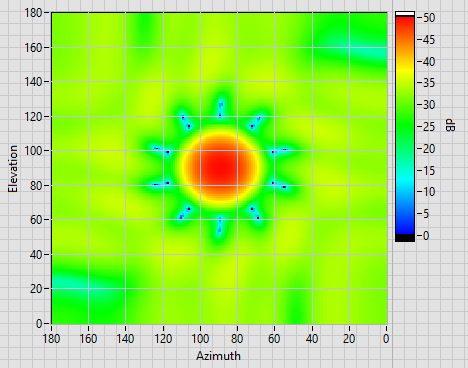
\includegraphics[keepaspectratio, width = 0.45\textwidth]{Figures/Final1k.png}} &
%            \subfloat[Final Array 10kHz Response]{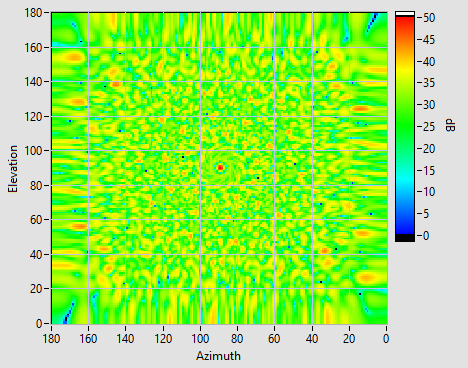
\includegraphics[keepaspectratio, width = 0.45\textwidth]{Figures/Final10k.png}}
%        \end{tabular}
%        \caption{Final Array 3D Responses}
%        \label{fig:Final 3D Response}
%        \end{figure}
        
    Now that the design had been finalised and deemed appropriate for the microphones and use case it was modelled in Solidworks as can be seen in Figure \ref{fig:Final Array} (a) due to the complex geometry of the design it was laser-cut out of 6mm plywood in four separate pieces and glued together. The design allows for the microphones to be screwed directly into their correct position with a much greater accuracy than if it was hand-made, this results in much tighter geometry tolerances and therefore higher accuracy beamforming.

    A lot of considerations were made when modelling the array for the best possible performance, one of the biggest issues with microphone arrays is noise and conflicting signals causing interference with the expected signals generally known as reverberation, this results in conflicting information being returned by the array. To avoid the problems of reverberation as much of the array surface area between microphones was removed to avoid reverberation from sound bouncing back off of the wooden surface whilst still keeping enough structural rigidity. Around the whole array several small holes were cut out for easier cable management and a flat spot on the top for a level as for accurate results the array must be level.

        \begin{figure} [H]
        \centering
        \begin{tabular}{cc}
            \subfloat[Solidworks Geometry Render]{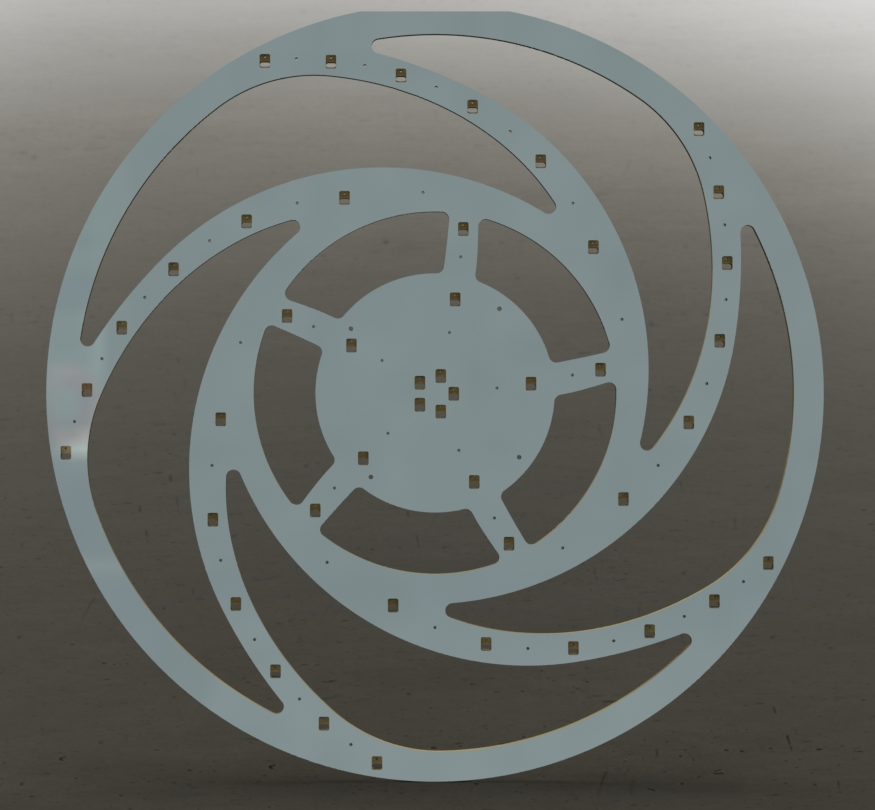
\includegraphics[keepaspectratio, width = 0.45\textwidth]{Figures/SolidWorks Array.png}} &
            \subfloat[Real Array]{\includegraphics[keepaspectratio, width = 0.45\textwidth]{Figures/Real Array.png}}
        \end{tabular}
        \caption{Final Array}
        \label{fig:Final Array}
        \end{figure}
    
%%%%%%%%%%%%%%%%%%%%%%%%%%%%%%%%
\subsubsection{Design Comparison} \label{sec:Design Comparison}

    Below in Figure \ref{fig:Comparison 3D Response} a comparison of the first testing array and final design at 3kHz. As expected the final design has much lower side-lobe levels and smaller main-lobe giving the array higher resolution and a higher signal to noise ratio, a significant improvement over the original array. 
        
        \begin{figure} [H]
        \centering
        \begin{tabular}{cc}
            \subfloat[First Array 3kHz Response]{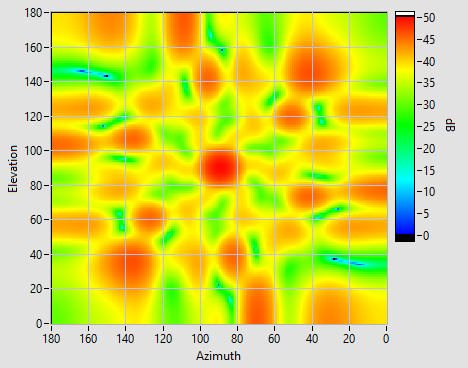
\includegraphics[keepaspectratio, width = 0.45\textwidth]{Figures/12mic3k.png}} &
            \subfloat[Second Array 3kHz Response]{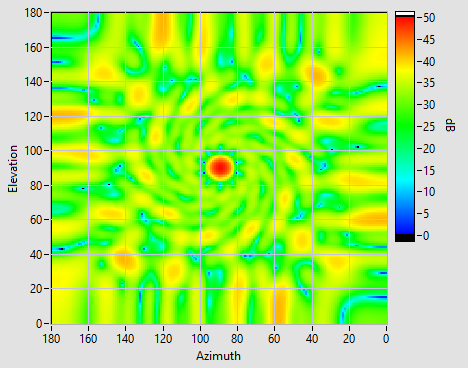
\includegraphics[keepaspectratio, width = 0.45\textwidth]{Figures/Final3k.png}}
        \end{tabular}
        \caption{Array Comparison 3D Responses}
        \label{fig:Comparison 3D Response}
        \end{figure}
        
%%%%%%%%%%%%%%%%%%%%%%%%%%%%%%%%
\subsection{Microphones} \label{sec:Microphones}
    Before the wide availability of MEMS (MicroElectrical-Mechanical System) Microphones arrays were required to be set up with conventional analog microphones, this made the costs and size for arrays very expensive, large and heavy, limiting the widespread availability of this technology with such a high barrier to entry without even considering the data acquisition. With the now every-growing mobile phone industry MEMS Microphones are incredibly cheap starting at less than a dollar each, this allows for large arrays to be built for very low costs \citep{San17}. The SPW2430 MEMS microphones were selected for my array, they boast a flat frequency response between 100Hz and 10kHz making them a perfect pairing for the microphone array \citep{Ada}, they are cost efficient and can be bought directly from many local and international distributors on breakout boards that are able to be directly wired into the National Instrument hardware as they have an analog DC output that is easily digitized for analysis and post processing.
%%%%%%%%%%%%%%%%%%%%%%%%%%%%%%%%
\subsection{Data Acquisition} \label{sec:DAQ}

\subsubsection{First Array} \label{sec:First Design DAQ}
    The initial testing array consisted of 12 of the SPW2430 MEMS Microphones mounted on a large piece of cardboard. There were four NI 9232 C-series modules available for analog input in a NI cDAQ-9178 for data acquisition, at the time of the photos three of the c-series modules were being used for other projects. The NI 9232 C-series modules are designed for sound and vibration inputs and take in three signals each simultaneously, with built in anti-aliasing filters for the selected sample rates up to 102.4kHz per channel \citep{NI9232}. The NI cDAQ-9178 allows for the data acquisition from the NI-9232 modules and the synchronisation of the acquired data across multiple modules, it communicates with a computer via a USB for plug-and-play simplicity \citep{cDAQ9178}. Figure \ref{fig:TestSetup} and demonstration of how the components are put together.

    One of the most important outcomes taken from the initial testing of this array was the need for proper wiring, the wiring used can be seen in Figure \ref{fig:TestSetup} is a high gauge wire that comes with 3-wires in a flat ribbon with no shielding or way to prevent environmental electrical noise. This resulted in a lot of noise across all the channels and was something that must be changed for the next iteration.

    \begin{figure} [H]
        \centering
        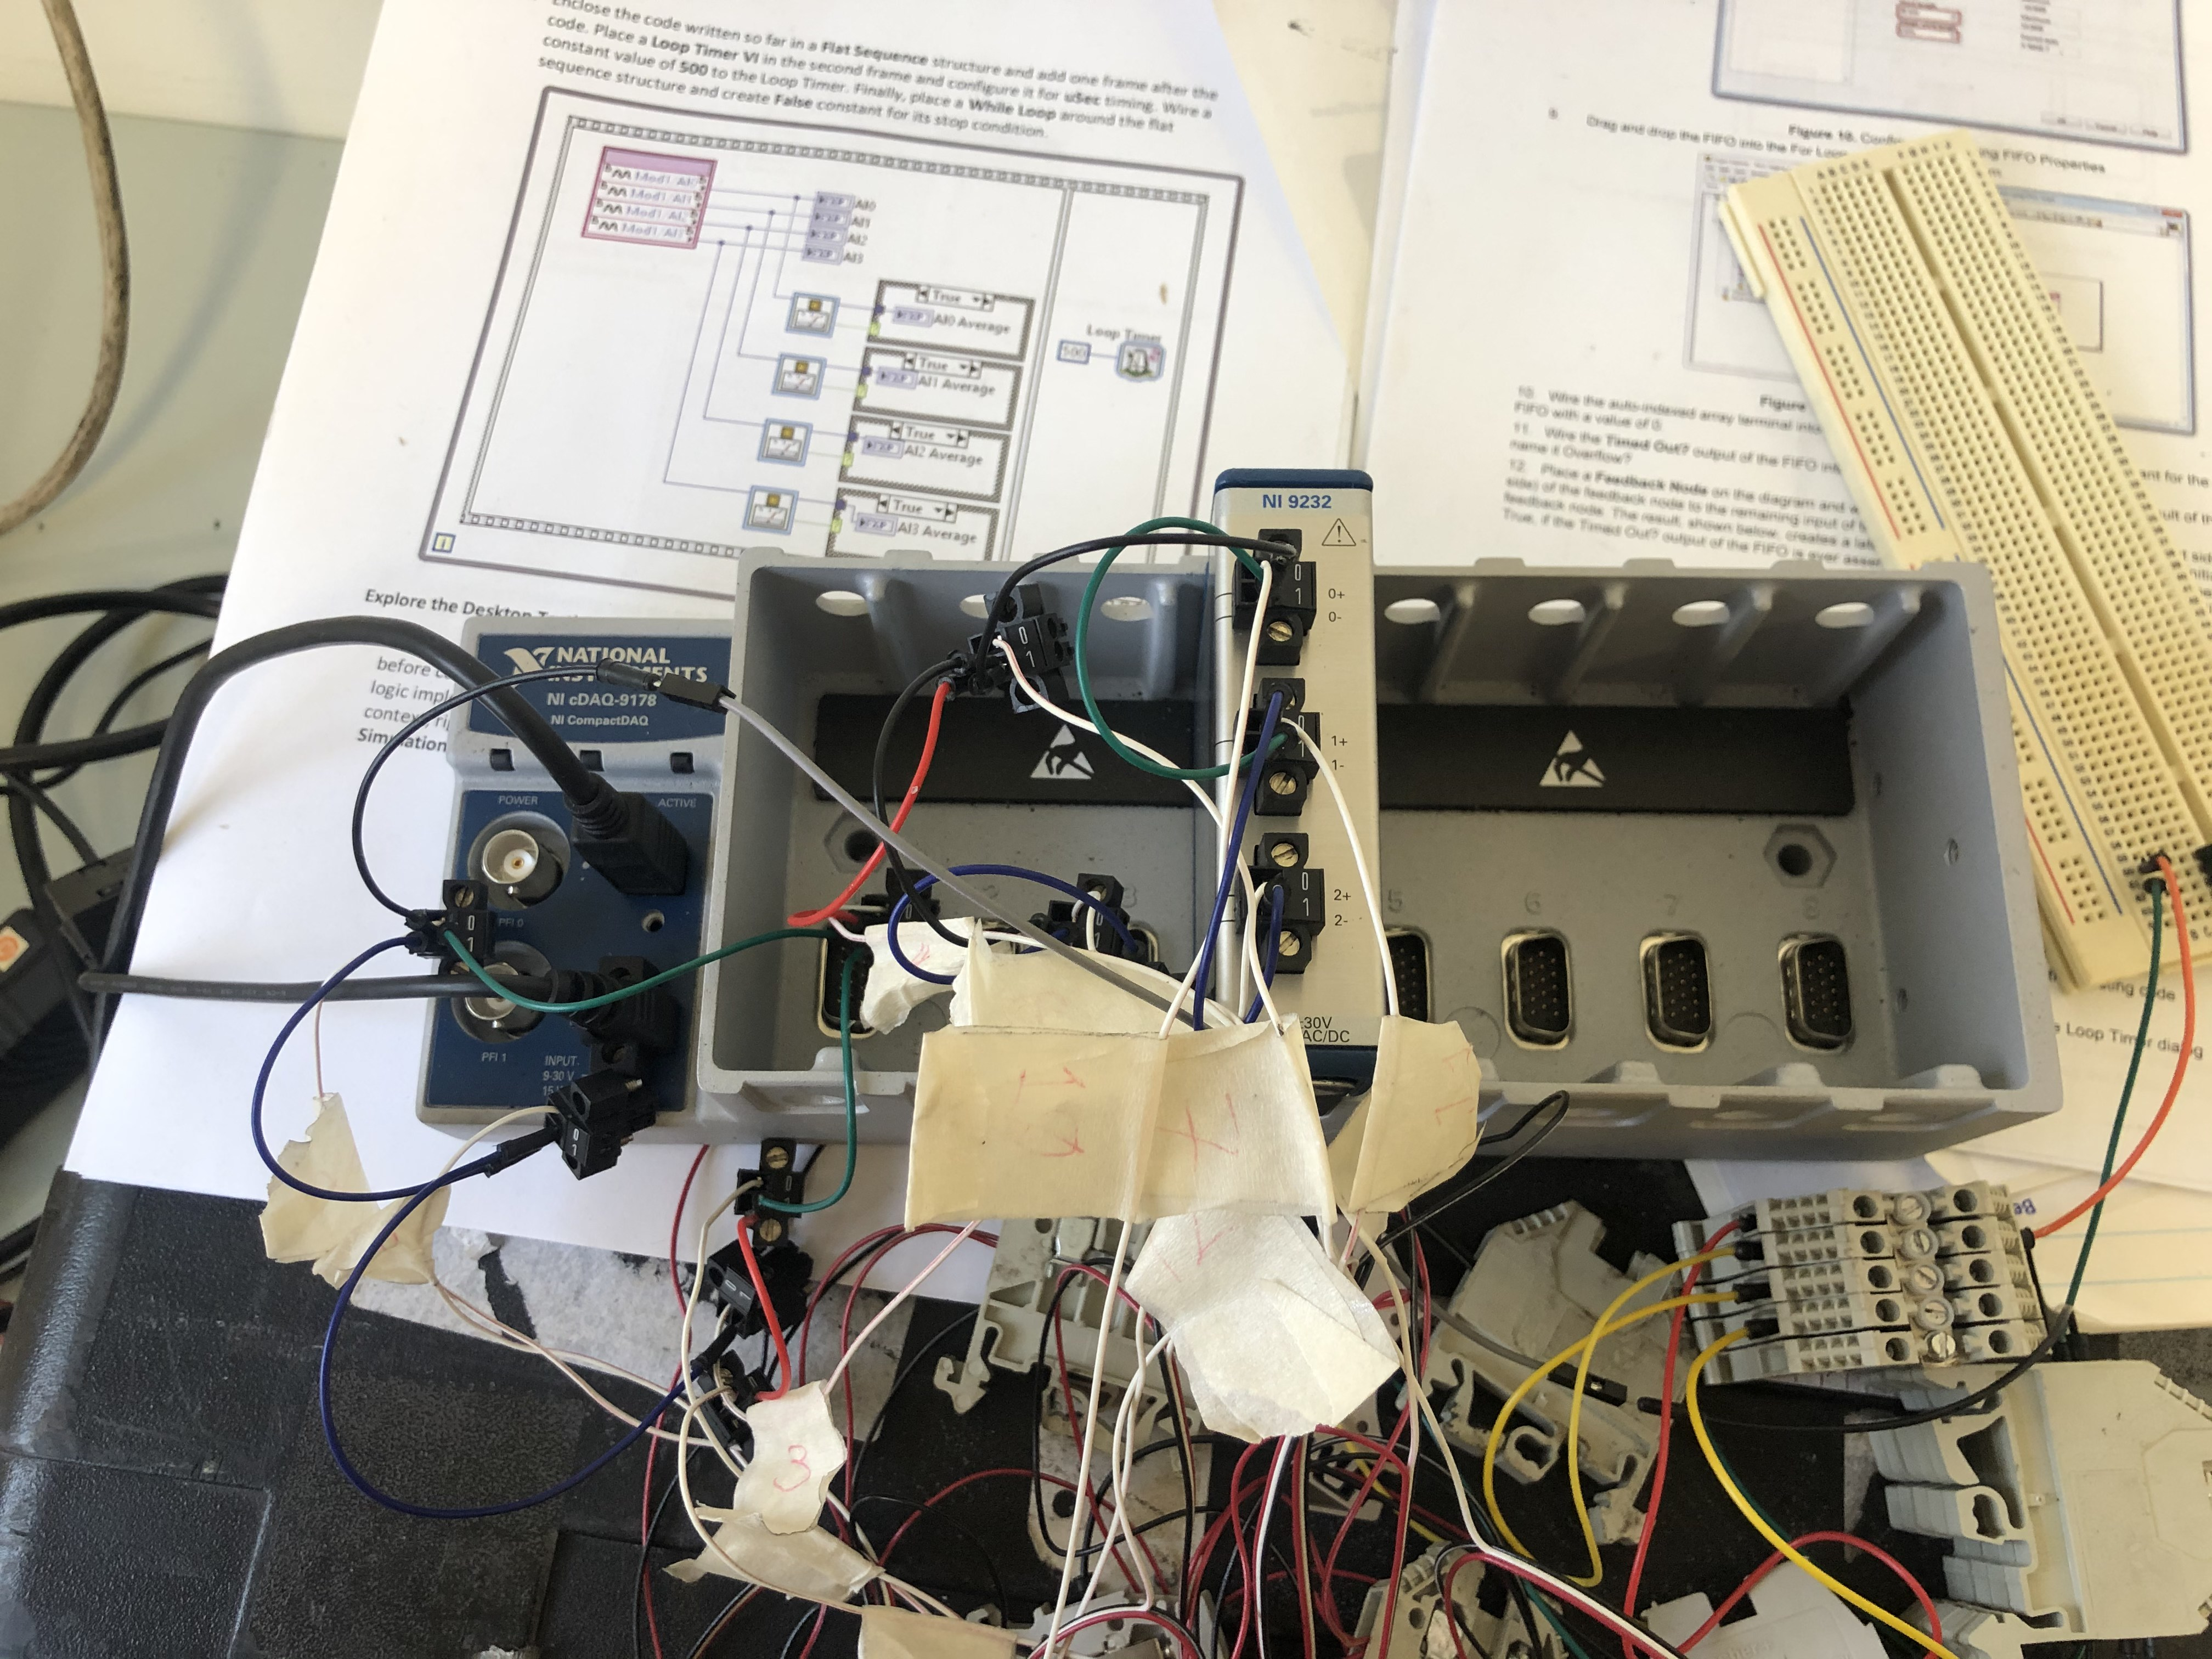
\includegraphics[keepaspectratio, width = 0.6\textwidth]{Figures/cDAQ.jpg}
        \caption{NI cDAQ with a single NI 9232 Installed and Wired Up}
        \label{fig:TestSetup}
    \end{figure}

\subsubsection{Second Array} \label{sec:Second Design DAQ}
    The second array was designed to be used with two NI cRIO-9036's Real Time Targets with FPGA's and 16 NI-9232 C-series Modules. This configuration would have allowed for up to 48 Channels of synchronised 102.4kHz input signals being processed on the cRIO's themselves with potential to move some processing to the FPGA. Due to unforeseen circumstances this hardware was made inaccessible and unavailable and a change of hardware was required. The hardware was changed back to the NI cDAQ-9178 and 8 NI-9229's C Series Modules, this allows for up to 24 synchronous channels of 50kHz sample rate \citep{NI9229}. Hence the final microphone array only consisted of 24 microphones with all processing taking place on an attached computer. As the array was designed for the use of 45 microphones spanning over 5 arms it had to be cut down, the inner 20 were microphones were chosen and then 4 of the 5 on the next ring of microphones as shown in Figure \ref{fig:FinalBuild}.
    
    \begin{figure} [H]
        \centering
        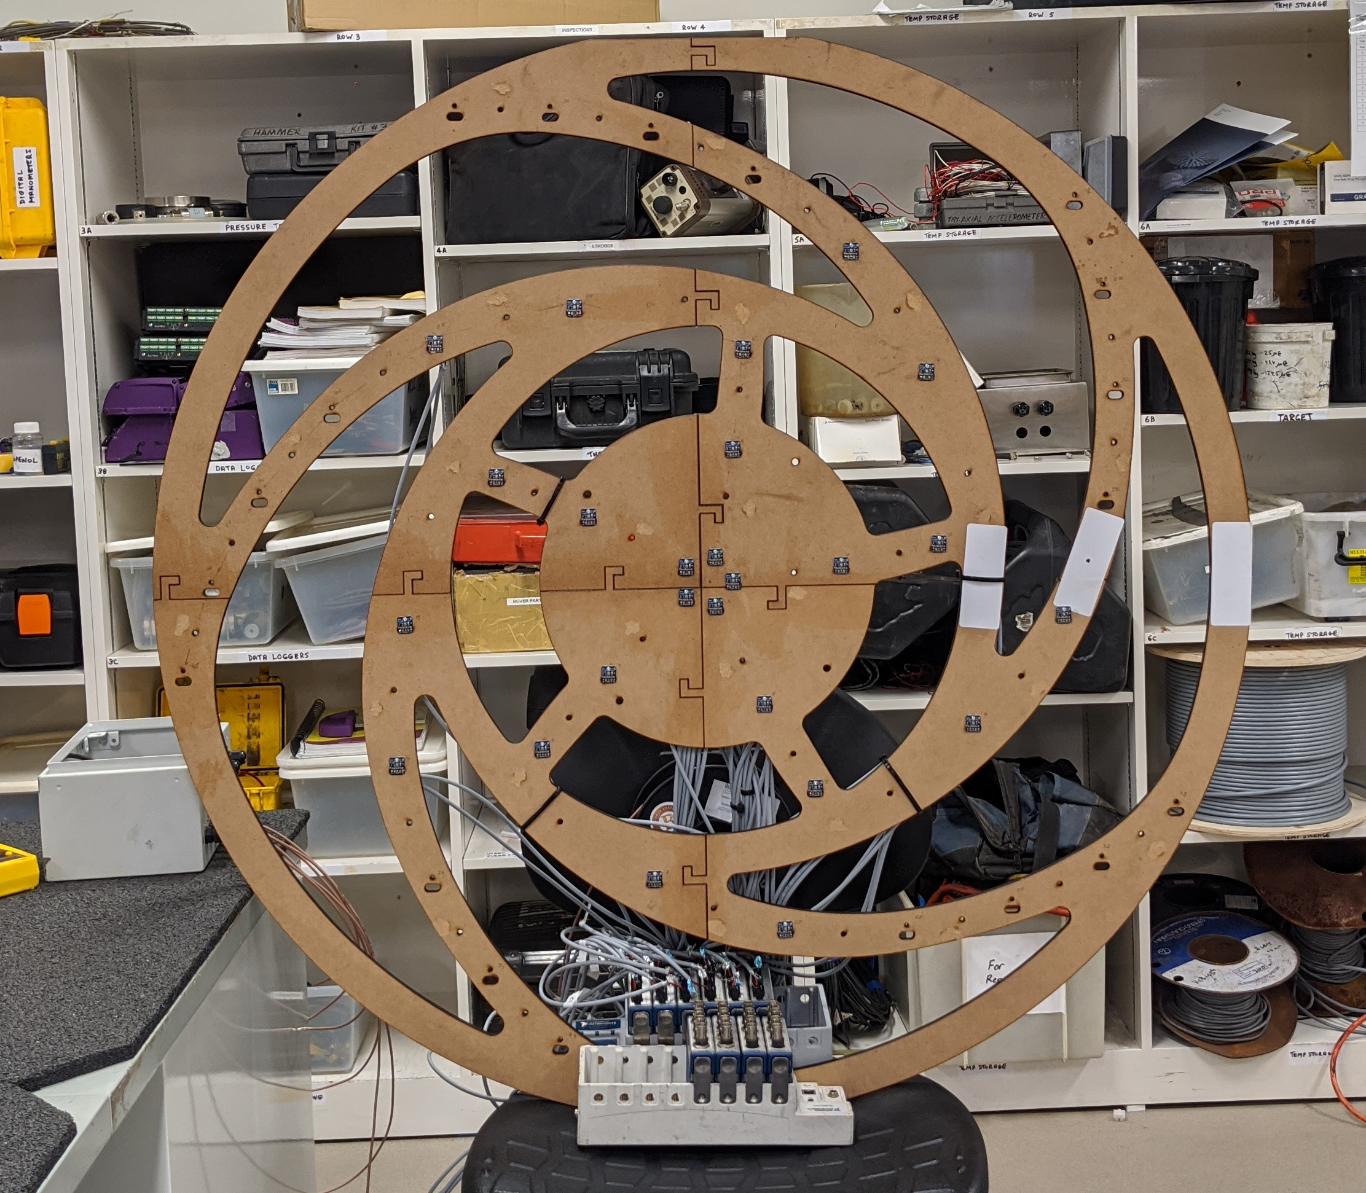
\includegraphics[keepaspectratio, width = 0.75\textwidth]{Figures/FinalArrayBuilt.png}
        \caption{Final Microphone Array with 24 Microphones}
        \label{fig:FinalBuild}
    \end{figure}

    In attempt to prevent the problem of noise from the external electrical environment as was present in the initial design due to the choice of wiring for this design each microphone had two separate shielded twisted pair cables. This allowed for a single twisted pair for the signal going back to the data acquisition card and a single twisted pair going back to power for each microphone. Once the cables were properly shielded it resulted in a dramatic reduction in noise. Figure \ref{fig:FinalWiring} shows the microphones all cabled and screwed in. 

    \begin{figure} [H]
        \centering
        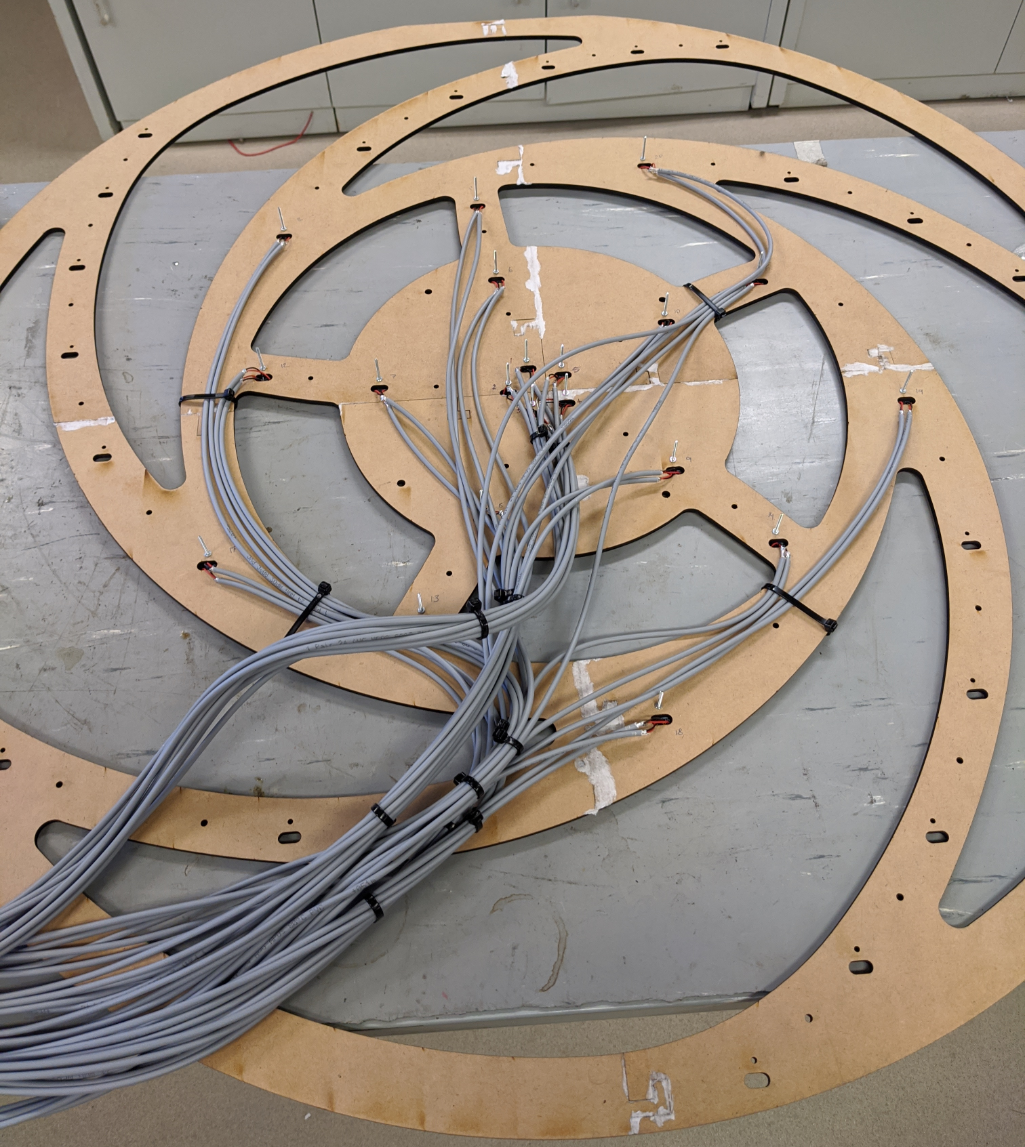
\includegraphics[keepaspectratio, width = 0.5\textwidth]{Figures/FinalArrayWiring.png}
        \caption{Final Microphone Array Wiring}
        \label{fig:FinalWiring}
    \end{figure}
    
    A comparison of the intended final array and the used final array is shown in Figure \ref{fig:FreqResponseComparison}, the designed final array has a much better response as would be expected with almost double the microphones but the final microphone array has an adequate response and is still preferred to the first design.
    
    \begin{figure} [H]
        \centering
        \begin{tabular}{cc}
            \subfloat[Designed Final Microphone Array]{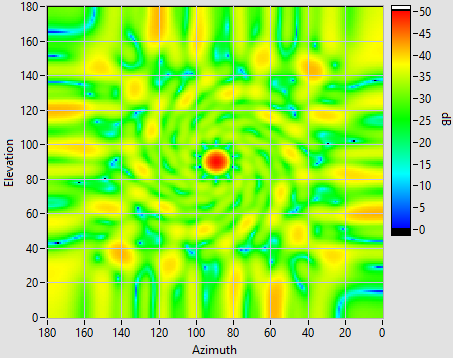
\includegraphics[keepaspectratio, width = 0.45\textwidth]{Figures/45MicFreqResponse3k.png}} &
            \subfloat[Final Microphone Array]{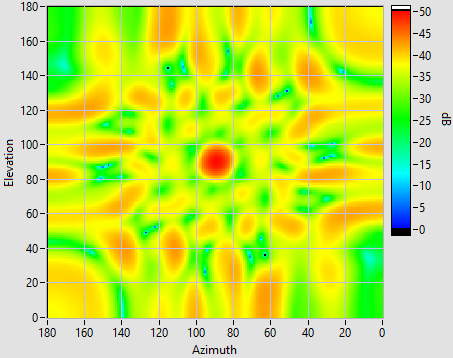
\includegraphics[keepaspectratio, width = 0.45\textwidth]{Figures/24MicFreqResponse3k.png}}
        \end{tabular}
        \caption{Comparison of Frequency Responses at 3kHz}
        \label{fig:FreqResponseComparison}
    \end{figure}
    
%%%%%%%%%%%%%%%%%%%%%%%%%%%%%%%%
\newpage
\section{Application to Machine Defects} \label{sec:Machine Defects}

Vibration analysis is used to evaluate the condition of machinery and determine whether defects due to misalignment, bearing degradation, looseness or any other potential factors that could be present. These defects generally cause vibration or impacting within the shaft or bearing housing that can be analysed and diagnosed, diagnosis requires the measurement of the vibration, velocity or displacement of the shaft or bearing housing over a period of time so that the time waveform and the frequency spectrum can be obtained and then analysed. Instead of using an accelerometer to measure the vibration it is possible to use a microphone as these defects generate noise the same way they generate vibration, with an array of microphones this will give the ability to pinpoint certain defects of machinery.

Focusing on the frequency spectrum as the features and patterns present can be directly related to those that would be picked up by a microphone array and therefore located. When analysing spectrums for defects there are various patterns and features to look out for that are typical of certain fault cases, some of these can be:

\begin{itemize}
    \item Harmonic patterns
    \item Periodic events
    \item Sidebands
    \item Separation of close frequencies
\end{itemize}

Harmonic patterns are multiples of a specific frequency for example if there is a frequency at 25Hz it's harmonics would be 50Hz, 75Hz, 100Hz and so on. The first frequency (25Hz) is known as the fundamental frequency.
Harmonics can be synchronous, sub-synchronous or non-synchronous. Synchronous includes the running speed frequency and all of its harmonics, sub-synchronous is below the running speed frequency and non-synchronous are all the frequencies between harmonics, all of these can indicate different types of faults. Common reasons for synchronous energy in the spectrum is imbalance, misalignment, looseness, blade/vane pass frequencies or gears, for sub-synchronous energy is commonly due to other machinery, hydraulic instability, or cage frequencies of bearings and for non-synchronous energy energy is commonly due to rolling element bearing defects, resonances, cavitations or other components and machines \citep{Mob20}. \hl{hand book}

Sidebands occur when there are two equally space frequencies on the higher and lower side of a frequency for example if there is a frequency a 125Hz and two more frequencies at 130Hz and 120Hz these two frequencies would be called sidebands, specifically 10Hz sidebands. A single frequency with sidebands in a time waveform would look like amplitude modulation, and if there are also harmonics with sidebands present this would look like amplitude modulation with a distorted fundamental carrier wave. Common reasons for the appearance of sidebands are gear tooth wear, gear backlash, motor rotor faults or bearing ball defects \citep{Mob20}. \hl{handbook}

Knowing these common occurring defects of machinery that can be identified through the frequency spectrum with the addition of a microphone array beamforming with the MUSIC algorithm it is possible to determine locations of certain defects by targeting that particular set of frequencies, as well as this the sound can then be extracted from that location for further analysis. 

%%%%%%%%%%%%%%%%%%%%%%%%%%%%%%%%
\newpage
\section{Testing} \label{sec:Lab Testing}
%%%%%%%%%%%%%%%%%%%%%%%%%%%%%%%%
\subsection{Early Testing of First Design} \label{sec:First Array Testing}
    Early testing  involved myself whistling in-front of the array, but this did give promising results. For the final testing of the first design I was standing above the microphone array whistling while acquiring one second of data, using the delay and sum algorithm on this one produced the heat-map shown in Figure \ref{fig:RealWhistle}. This result accurately estimated the source to be right at the top of the array in the centre which is accurate to where I was, also present are two relatively major side-lobes in the bottom right quadrant of the heat-map.
    
    \begin{figure} [H]
        \centering
        \includegraphics[keepaspectratio, width = 0.6\textwidth]{Figures/RealWhistle.png}
        \caption{Result of Whistle testing}
        \label{fig:RealWhistle}
    \end{figure}
    
    After performing a Fourier transform on the signal it was found that my whistle frequency was 1675Hz this is information as well as its spatial location was required to test the result in simulation and 3D frequency response for verification. Knowing the location and the frequency a 3D Frequency response was setup with those parameters producing Figure \ref{fig:RealWhistleFreq}. As can be this produced a very similar looking heat-map which would indicate that the algorithm and hardware are both working on the test array as that would be the only way to produce such similar results. The main-lobe and side-lobes all look nearly identical between the real test and the 3D Frequency Response.
    
    \begin{figure} [H]
        \centering
        \includegraphics[keepaspectratio, width = 0.6\textwidth]{Figures/RealWhistle3DFreqResp.png}
        \caption{Whistle test 3D Frequency Response}
        \label{fig:RealWhistleFreq}
    \end{figure}
    
    To further validate the results from the test run the parameters were again used in the simulation. Figure \ref{fig:RealWhistleSim} shows the results from this. Again showing the same and very promising results as the 3D Frequency response as was expected.
    
     \begin{figure} [H]
        \centering
        \includegraphics[keepaspectratio, width = 0.6\textwidth]{Figures/RealWhistleSim.png}
        \caption{Whistle test Simulation}
        \label{fig:RealWhistleSim}
    \end{figure}

    This whistle test and following simulations validated the array design and that it was working with delay and sum algorithm, though due to the external electrical noise in the wiring and the small number of microphones no more testing was performed or required and moving onto the design of a larger array and improved algorithms were the next steps.
    
%%%%%%%%%%%%%%%%%%%%%%%%%%%%%%%%
\newpage
\subsection{Final Design Testing} \label{sec:Second Array Testing}
    Before the final testing took place the array was tested to at the least be able to determine the correct side of the array a signal was arriving from, these results can be found in Appendix \ref{app: Testing Figures}. Following the success of the array to estimate the correct general location of incoming signals further test cases as described in the following sections were carried out.
%%%%%%%%%%%%%%%%%%%%%%%%%%%%%%%%
\subsubsection{Design Verification} \label{sec:Design Verification Testing}
    To verify the accuracy and performance of the microphone array testing was performed in the lab using a speaker and a laser distance measurer. There were two tests performed one with a speaker at 70 Degrees Azimuth and the other with the speaker at 170 Degrees Azimuth from leftmost side of the array both at the centre of Elevation, these angles were calculated with basic trigonometry using the laser distance measurer, the 70 Degree test was 4m away from the origin of the array whilst the 170 Degree test was 3m from origin.

    Figure \ref{fig:array verification} displays the results of the delay-and-sum algorithm to both of the test, this algorithm was chosen for the purpose of verifying the array due to it being much less error prone than MUSIC with less need for user input and has previously been tested and shown to work with a real array. The results show that the array does indeed operate as expected as well as the algorithm. The 70 Degree test was close to exact along the azimuth and was estimated to be a few degrees above its true elevation. Inaccuracies begin to show at the edge of the array for the 170 Degree test with the azimuth estimation being around 10 Degrees off but the elevation estimation was as expected.
    
    If we refer back to Figure \ref{fig:2DResponseSteered} the reason for the inaccuracies at the edge of the array can be explained, as the array is steered towards the edge the main-lobe of the 2D frequency response becomes larger in the exact same way as is seen in the 170 Degree test. This can be attributed all the way back to Eqn. \ref{eq:TDOA} where it was determined that the time difference of arrival for signals is a cosine function and hence as the angle of arrival approaches either 0 or 180 Degrees the time difference of arrival between microphones becomes increasingly smaller and increasingly difficult to separate between angles creating the large main-lobes as steering towards the edges of the array as seen in Figure \ref{fig:2DResponseSteered} and \ref{fig:array verification}, this will occur in both the delay-and-sum and the MUSIC algorithm as it comes to the characteristics of sound waves. To show the difference between two points on an array results from two calculations using Eqn. \ref{eq:TDOA} are shown in Table \ref{tab:TimeDelay}, this table shows the difference in the time difference of arrival when moving 1 degree across the azimuth towards centre from both 40 Degrees and 170 Degrees, the difference in time delay being much smaller when at 170 Degrees.

    \begin{table}[H]
        \centering
        \ra{1}
        \caption{Array Time Delay Comparisons} 
        \begin{tabular}{cccc}
            \toprule
            Angle 1 & Angle 2 & $\Delta\tau_{1,2}$ & $\Delta$ \%$_{1,2}$ \\
            \midrule
            40 & 39 & $1.616e$-$05$ & - \\
            170 & 169 & $4.632e$-$06$ & -28.66 \\
            \bottomrule
        \end{tabular}
        \label{tab:TimeDelay}
    \end{table}
    
    \begin{figure} [H]
        \centering
        \begin{tabular}{cc}
            \subfloat[70 Degree Azimuth Test]{\includegraphics[keepaspectratio, width = 0.45\textwidth]{Figures/20DegDAS.png}} &
            \subfloat[170 Degree Azimuth Test]{\includegraphics[keepaspectratio, width = 0.45\textwidth]{Figures/10DegDAS_Test.png}}
        \end{tabular}
        \caption{Array Verification Test}
        \label{fig:array verification}
    \end{figure}
    
%%%%%%%%%%%%%%%%%%%%%%%%%%%%%%%%
\subsubsection{Algorithm Comparison} \label{sec:Algorithm Comparison Testing}
    The next stage of testing involved testing and comparing the accuracy of both the delay-and-sum and MUSIC algorithm by comparing the results to an identical sound source. Again using the laser distance measurer a speaker was placed at 47 Degrees Azimuth and centre of the Elevation playing a 1871Hz tone.

    For both of the results shown in Figure \ref{fig:algorithm comparison} the algorithms were using the exact same 0.1s snippet of sound, the MUSIC algorithm just processed for the exact 1871 frequency whilst delay and sum is required to process the full snippet. The delay and sum resulted in a 3 Degree accuracy to the true source location and the MUSIC algorithm resulted in a 2 Degree accuracy, the resolution of the MUSIC algorithm is much higher though as well as having a significantly lower noise and number of side-lobes present. As well as showing better resolution and accuracy the MUSIC algorithm was over 10 times as fast as the delay and sum algorithm further cementing its place for determine the location of specifically chosen frequencies.

    \begin{figure} [H]
        \centering
        \begin{tabular}{cc}
            \subfloat[Delay and Sum Algorithm]{\includegraphics[keepaspectratio, width = 0.45\textwidth]{Figures/47DegDas01s.png}} &
            \subfloat[MUSIC Algorithm]{\includegraphics[keepaspectratio, width = 0.45\textwidth]{Figures/47DegMUSIC01s.png}}
        \end{tabular}
        \caption{Real Algorithm Comparison to 1871Hz Signal}
        \label{fig:algorithm comparison}
    \end{figure}

%%%%%%%%%%%%%%%%%%%%%%%%%%%%%%%%
\subsubsection{Defect Detection} \label{sec:Defect Detection Lab Testing}

    Now to verify the ability of the array to differentiate different noise and spatially locate them a simple test was performed in a lab environment. To the right hand side 3m from the array a speaker was playing a loud 2.5kHz sinusoidal tone and in front of the array to the left 8m away was a turbine balance test rig running at 3000rpm, the purpose of the test was to see if it would be possible to differentiate the sources.

    Figure \ref{fig:mic signals lab test} shows the signals captured by the microphone array over a 4 second period. As can be seen in the frequency spectrum, there is a significant amount of noise in the sub 1kHz frequency range, a large spike at 2.5kHz, a small bunch of signals at 5kHz and 6kHz and more noise around 9-11kHz. As the lab was relatively quiet the peaks that appeared at 5kHz and 6kHz were assumed to be coming from the balancing test rig, Figure \ref{fig:zoom mic signals lab test} provides a closer look at some of the assumed signals from the balancing test rig.
    
    \begin{figure} [H]
        \centering
        \includegraphics[keepaspectratio, width = \textwidth]{Figures/Raw Sound Waves.png}
        \caption{Microphone Signals}
        \label{fig:mic signals lab test}
    \end{figure}
    
    \begin{figure} [H]
        \centering
        \includegraphics[keepaspectratio, width = \textwidth]{Figures/Zoomed Sound Waves.png}
        \caption{Zoomed Microphone Signals}
        \label{fig:zoom mic signals lab test}
    \end{figure}
    
    In the following Figure \ref{fig:defect detection lab test results} it is shown that the array succeeded in differentiating the signal source locations and identified the correct locations for the signals. The color scale for the intensity map was changed for Figure \ref{fig:defect detection lab test results} for less confusion when interpreting the result, instead of showing all side-lobes and the main-lobe this scale only shows the main lobe and highest side-lobes if they are present. In Figure \ref{fig:defect detection lab test results}(a) a single frequency of 2474Hz was searched for using the MUSIC algorithm and for Figure \ref{fig:defect detection lab test results}(b) a set of frequencies was used to search for, these being: 4812Hz, 4870Hz, 4921Hz, 6080Hz, and 6090Hz, these being the prominent signals that are present in Figure \ref{fig:zoom mic signals lab test}. As shown this method of differentiating signals by selecting certain frequencies worked well, the 2.5kHz signal was located  accurately though the estimated area is relatively large, on the other-hand the turbine balance test rig was estimated very precisely and accurately though there is a large level of side-lobes creating some uncertainty within the results. Impressively the array could pick out the turbine test rig using the particular frequencies even when they were barely above the noise floor of the environment.
    
    \begin{figure} [H]
        \centering
        \begin{tabular}{cc}
            \subfloat[2.5kHz Signal Location]{\includegraphics[keepaspectratio, width = 0.45\textwidth]{Figures/2474Hz_ReColour.png}} &
            \subfloat[Turbine Balance Test Rig Location]{\includegraphics[keepaspectratio, width = 0.45\textwidth]{Figures/BalancingRig_ReColour.png}}
        \end{tabular}
        \caption{Differentiate signal testing results}
        \label{fig:defect detection lab test results}
    \end{figure}
    
    This test shows promising results with the array proving that is able to differentiate particular noise sources by frequency and even when the particular frequencies of interest are only just above the noise floor. As well this test has reinforced the potential of the microphone array for finding defects in machine by using a particular set of frequencies to pin-point spatially.

%%%%%%%%%%%%%%%%%%%%%%%%%%%%%%%%
\newpage
\subsection{Site Testing} \label{sec:Site Testing}

    Site testing was conducted at a local power-station that had been experiencing issues with one of their steam-driven turbines. The turbine had been suffering from a hammering-like noise originating from an unknown source. The primary aims of this testing was first to evaluate the effectiveness of the array in a loud industrial environment with operating machinery and the second aim was to determine where the noise was originating from and what was causing it.
    
    Figure \ref{fig:turbine} shows an overview of the general turbine layout with labelled cylinders and bearings for future reference.

    \begin{figure} [H]
        \centering
        \includegraphics[keepaspectratio, width = \textwidth]{Figures/LabelledTurbine.jpg}
        \caption{Typical 4 Cylinder Reheat Steam Turbine \citep{WWH}}
        \label{fig:turbine}
    \end{figure}

    % http://what-when-how.com/energy-engineering/steam-turbines-energy-engineering/

    The array with it's 24 microphones was brought onto site and placed at various points of the second Low Pressure Cylinder (LPB) close to where the noise was described to be originating from by the client. Data was taken from the unit generating the noise and then at the same locations on the a second unit that had not been generating the noise to provide a comparison of the noise characteristics of each unit. Measurements were taken at the casing between bearing's 8 and 9, in the middle of the LPB Cylinder and at the casing between bearing 6 and 7 to try and gain a full insight to the full soundscape of the LPB Cylinder. Pictures taken from the perspective of the microphone array of all these locations can be found in Appendix \ref{app:Site Testing}.

    \subsubsection{Acquired Data} \label{sec:Site Acquired Data}

    Firstly, looking at a comparison of the spectrums and waveforms received at both of the turbines. Figure \ref{fig:U5 Signal} and \ref{fig:U6 Signal} show the spectrum and time waveform of the bad and good turbines respectively. When comparing the signals look nearly identical, interestingly the good turbine was quite a bit louder than the bad turbine producing a much higher peak in the time waveform and frequency amplitudes in the spectrum. 

    The primary features of both spectrums is the series of harmonics, the fundamental frequency of both turbines is 50Hz as they are running at 3000rpm, hence the spectrum is filled with harmonics of the fundamental frequency, more specifically odd harmonics, 150Hz, 250Hz, 350Hz, etc. . 

    \begin{figure} [H]
        \centering
        \includegraphics[keepaspectratio, width = \textwidth]{Figures/U5_LPB.png}
        \caption{Spectrum and Time Waveform Centre of LPB Problem Unit}
        \label{fig:U5 Signal}
    \end{figure}

    \begin{figure} [H]
        \centering
        \includegraphics[keepaspectratio, width = \textwidth]{Figures/U6_LPB.png}
        \caption{Spectrum and Time Waveform Centre of LPB Good Unit}
        \label{fig:U6 Signal}
    \end{figure}

    Unfortunately testing did not go as well as I would have hoped, beamforming with the array was unable to locate any sound sources with delay and sum or even any individual or sets of frequencies using MUSIC. Figure \ref{fig:TurbineSinglePeriod} shows a comparison of the two turbines waveforms over a single period. 

    \begin{figure} [H]
        \centering
        \begin{tabular}{c}
            \subfloat[Problem Unit Bearing 8]{\includegraphics[keepaspectratio, width = \textwidth]{Figures/U5Bearing89_Period.png}} \\
            \subfloat[Good Unit Bearing 8]{\includegraphics[keepaspectratio, width = \textwidth]{Figures/U6Bearing89_Period.png}}
        \end{tabular}
        \caption{Turbine Single Period Comparison}
        \label{fig:TurbineSinglePeriod}
    \end{figure}
    
    Both of the time waveforms shown in Figure \ref{fig:TurbineSinglePeriod} are very similar but there is one notable problem with both of these in regards to beamforming, there is absolutely no time difference of arrival between microphones, which is the basis that allows all beamforming to take place. This problem causes the array to estimate the sound source as originating from the exact center of the array. Figure \ref{fig:Beamforming Results U5 LPB} displays the results for beamforming with both the delay-and-sum and MUSIC algorithm at the center of the problem turbine's LPB cylinder. 
    
    \begin{figure} [H]
        \centering
        \begin{tabular}{cc}
             \subfloat[DAS Algorithm]{\includegraphics[keepaspectratio, width = 0.45\textwidth]{Figures/U5Cyl_DAS.png}}&
             \subfloat[MUSIC Algorithm 2kHz - 3kHz]{\includegraphics[keepaspectratio, width = 0.45\textwidth]{Figures/U5Cyl_MUSIC.png}}
        \end{tabular}
        \caption{Beamforming Results LPB Cylinder Problem Unit}
        \label{fig:Beamforming Results U5 LPB}
    \end{figure}
    
    As expected the results in Figure \ref{fig:Beamforming Results U5 LPB} from beamforming with both algorithms returned similar results with estimated sound source being in the dead center of the array. This result was constant with all locations tested from both turbines, no matter the frequencies searched for using MUSIC, the estimated sound source was always in the dead center of the array.
    
    Looking at the signals in Figure \ref{fig:U5 Signal} and \ref{fig:U6 Signal} it would be assumed that the signals are indeed coming from directly in the centre of the array as all the signals are arriving at the same time, though due to the many different testing locations around the turbine floor and the signal being the same at all locations the sound cannot realistically be coming from a point directly in the centre of the array at all points, there are two main thoughts as to the reasons this is happening. The first theory is that the cylinder itself and the bearing casings of the turbine are acting as one large loudspeaker, this would be amplifying the noise over the whole turbine, this fits the signal being synchronised on all microphones as the sound would be from directly in front of all microphones. The second theory is that due to the environment of the power station that the reverberation off of the surrounding structure and plant is causing the signal to be coming from all directions at once and hence the microphone signals all being synchronised.
    
%%%%%%%%%%%%%%%%%%%%%%%%%%%%%%%%
\newpage
\section{Conclusion} \label{sec:Conclusion}
    %\hl{restatement of aims; achievement of aims; summary of relevance of research; restatement of results and brief evaluation}
    %\hl{more industrial testing, fpga, more microphones etc would be better}
    
    The primary aims of this project were to build a working acoustic beamforming array that would be able to locate and detect particular sounds in noisy environments as well as being able to extract the signal from the particular location. Throughout this project I achieved all of these aims by building a working acoustic beamforming  array that successfully located individual sounds out of a noisy test environment, though unfortunately was not able to locate sounds in the testing performed on-site. 
    
    My research into the area of beamforming array provided great insight into audio and digital signal processing, with this and the aid of my learning in LabVIEW development I was able to evaluate many different geometries,  algorithms and processing methods using the software I developed for simulation and found the MUSIC algorithm as being the most suitable and applicable to the purpose of locating and identifying defects in machinery when used to find a particular or set of frequencies.
    
    Using the acoustic array I designed with the Underbrink equations I found it was very capable of locating individual sound sources out of a noisy environment using the MUSIC algorithm, by searching for an individual frequency or a set of frequencies, this was shown by accurately differentiating and locating both a small turbine test-rig and speaker that were running simultaneously. Disappointingly the acoustic array when tested on in-service turbines at a local power-station was unable to beamform effectively at any location on the turbine-floor, this is thought to be due to either the whole casing of the turbine acting as a loud-speaker, an overwhelming amount of reverberation or a combination of both.
    
    In conclusion, with further testing on more and different plant as well as in different environments that this acoustic array could be used for the purpose of identifying and locating defects on machinery with further fine-tuning, refinement and understanding of sound propagation in industrial environments.
\newpage
%%%%%%%%%%%%%%%%%%%%%%%%%%%%%%%%
\bibliographystyle{harvard}
\bibliography{main} % This is the .bib file where the bibliography database is stored

\newpage
\appendix
\captionsetup[figure]{list=no}
\section{Time Log Graphic}

\newpage
\section{Reflection}
    \hl{A full extract of the stage 1 Engineers Australia professional engineers competencies are available online via the EA website. The intent of this section is for you to consider and comment on your personal journey through the degree and the acquisition of the competencies covered in your program.  Many engineering students commence as recent school leavers, and in the brief time at campus undergo a remarkable growth in attitude.  Using the lens of EA stage 1 competencies, this section is asking you to consider predominantly the section 3 personal and professional attributes and how your view on these might have changed in the last 4-5 years}
    
\newpage
\section{Simulation Figures} \label{app:Sim}
    \begin{figure}[H]
        \centering
        \includegraphics[keepaspectratio, width = \textwidth]{Figures/SimSignalCentre.png}
        \caption{Array of signals when Steered to the Centre of the Array}
    \end{figure}
    \begin{figure}[H]
        \centering
        \includegraphics[keepaspectratio, width = \textwidth]{Figures/SimSignalCentreSum.png}
        \caption{Array of signals at Centre Summed and Normalised}
    \end{figure}
    \begin{figure}[H]
        \centering
        \includegraphics[keepaspectratio, width = \textwidth]{Figures/SimSignalLocation.png}
        \caption{Array of signals when Steered to the Source Location}
    \end{figure}
    \begin{figure}[H]
        \centering
        \includegraphics[keepaspectratio, width = \textwidth]{Figures/SimSignalLocationSum.png}
        \caption{Array of signals at Source Location Summed and Normalised}
    \end{figure}

\section{Geometry Investigation} \label{app:Geom Invest}
\subsection{Geometries} \label{app:Geometries}
    \begin{figure} [H]
    \centering
    \begin{tabular}{cc}
        \subfloat[5 Arms, 45 Microphones, $v=\frac{2.9795 \pi}{8}$]{\includegraphics[keepaspectratio, width = 0.4\textwidth]{Figures/5Arms.png}} &
        \subfloat[6 Arms, 48 Microphones, $v=\frac{2.9795 \pi}{8}$]{\includegraphics[keepaspectratio, width = 0.4\textwidth]{Figures/6Arms.png}} \\
        \subfloat[7 Arms, 42 Microphones, $v=\frac{5}{16}$]{\includegraphics[keepaspectratio, width = 0.4\textwidth]{Figures/7Arms.png}} &
        \subfloat[8 Arms, 48 Microphones, $v=\frac{5}{16}$]{\includegraphics[keepaspectratio, width = 0.4\textwidth]{Figures/8Arms.png}} \\
        \multicolumn{2}{c}{\subfloat[9 Arms, 45 Microphones, $v=\frac{5}{16}$]{\includegraphics[keepaspectratio, width = 0.4\textwidth]{Figures/9Arms.png}}}
    \end{tabular}
    \caption{Series of tested microphone array geometries}
    \label{fig:Testing Geometries}
    \end{figure}
\subsection{Frequency Responses}\label{app:frequencies}
    \begin{figure} [H]
    \centering
    \begin{tabular}{cc}
        \subfloat[5 Arms, 45 Microphones, $v=\frac{2.9795 \pi}{8}$]{\includegraphics[keepaspectratio, width = 0.4\textwidth]{Figures/4kHzFinalResponse.png}} &
        \subfloat[6 Arms, 48 Microphones, $v=\frac{2.9795 \pi}{8}$]{\includegraphics[keepaspectratio, width = 0.4\textwidth]{Figures/4kHz6ArmsResponse.png}} \\
        \subfloat[7 Arms, 42 Microphones, $v=\frac{5}{16}$]{\includegraphics[keepaspectratio, width = 0.4\textwidth]{Figures/4kHz7ArmsResponse5_16_angle.png}} &
        \subfloat[8 Arms, 48 Microphones, $v=\frac{5}{16}$]{\includegraphics[keepaspectratio, width = 0.4\textwidth]{Figures/4kHz8ArmsResponse5_16_angle.png}} \\
        \multicolumn{2}{c}{\subfloat[9 Arms, 45 Microphones, $v=\frac{5}{16}$]{\includegraphics[keepaspectratio, width = 0.4\textwidth]{Figures/4kHz9ArmsResponse5_16_angle.png}}}
    \end{tabular}
    \caption{3D Frequency Response Results}
    \label{fig:Geometry Results}
    \end{figure}

\section{Testing Figure} \label{app: Testing Figures}
\begin{figure} [H]
    \centering
    \begin{tabular}{cc}
        \subfloat[Left Side]{\includegraphics[keepaspectratio, width = 0.475\textwidth]{Figures/LeftSide.png}} &
        \subfloat[Right Side]{\includegraphics[keepaspectratio, width = 0.475\textwidth]{Figures/RightSide.png}} \\
        \multicolumn{2}{c}{\subfloat[Top Side]{\includegraphics[keepaspectratio, width = 0.475\textwidth]{Figures/TopSide.png}}}
    \end{tabular}
    \caption{Initial Calibration Results}
    \label{fig:Initial Calibration Results}
    \end{figure}
\section{Site Testing Locations} \label{app:Site Testing}
    \begin{figure}[H]
        \centering
        \includegraphics[keepaspectratio, width = \textwidth]{Figures/U5_LPB_8.png}
        \caption{Problem Unit Bearing 8}
    \end{figure}
    \begin{figure}[H]
        \centering
        \includegraphics[keepaspectratio, width = \textwidth]{Figures/U5_LPB_8_2.png}
        \caption{Problem Unit Bearing 8 Angle 2}
    \end{figure}
    \begin{figure}[H]
        \centering
        \includegraphics[keepaspectratio, width = \textwidth]{Figures/U5_LPB_7.png}
        \caption{Problem Unit Bearing 7}
    \end{figure}
    \begin{figure}[H]
        \centering
        \includegraphics[keepaspectratio, width = \textwidth]{Figures/U5_LPB_Centre.png}
        \caption{Problem Unit LPB Cylinder}
    \end{figure}
    \begin{figure}[H]
        \centering
        \includegraphics[keepaspectratio, width = \textwidth]{Figures/U6_LPB_8.png}
        \caption{Good Unit LPB Bearing 8}
    \end{figure}
    \begin{figure}[H]
        \centering
        \includegraphics[keepaspectratio, width = \textwidth]{Figures/U6_LPB_Centre.png}
        \caption{Good Unit LPB Cylinder}
    \end{figure}

\end{document}